\documentclass[pdflatex,sn-nature]{sn-jnl}

\usepackage{graphicx}
\usepackage{manyfoot}
\usepackage{amsmath,amssymb,amsfonts}
\usepackage{booktabs}
\usepackage{longtable}
\usepackage{multirow}
\usepackage{array}
\usepackage{tabularx}
\usepackage{url}
\usepackage{xcolor}
\usepackage[section]{placeins}

\raggedbottom

\begin{document}

\title[TIMELY Bench]{TIMELY Bench for Temporal Clinical Reasoning in Critical Care}

\author*[1]{\fnm{Haoyu} \sur{Wang}}\email{haoyu.7.wang@kcl.ac.uk}
\equalcont{These authors contributed equally: Haoyu Wang, Zitong Li, Linglong Qian, and Zina Ibrahim.}

\author[1]{\fnm{Zitong} \sur{Li}}\email{zitong.2.li@kcl.ac.uk}
\equalcont{These authors contributed equally: Haoyu Wang, Zitong Li, Linglong Qian, and Zina Ibrahim.}

\author[1]{\fnm{Linglong} \sur{Qian}}\email{linglong.qian@kcl.ac.uk}
\equalcont{These authors contributed equally: Haoyu Wang, Zitong Li, Linglong Qian, and Zina Ibrahim.}

\author[1]{\fnm{Zina} \sur{Ibrahim}}\email{zina.ibrahim@kcl.ac.uk}
\equalcont{These authors contributed equally: Haoyu Wang, Zitong Li, Linglong Qian, and Zina Ibrahim.}

\affil*[1]{\orgname{King's College London}, \orgaddress{\city{London}, \country{United Kingdom}}}

\abstract{Temporal clinical reasoning requires interpreting partially observed patient trajectories, yet most clinical AI benchmarks test static prediction, medical question answering, or workflow execution. Using MIMIC-IV ICU stays, we developed TIMELY Bench, an ICU benchmark aligning AKI, delirium, sepsis, and stroke on a 168-hour hourly grid with anchor-bounded multimodal EHR prompts spanning structured measurements, medications, procedures, clinical notes, and condition-specific observations. The frozen evaluation sample included 12,000 instances from 9,587 ICU stays, expanded to 53,070 \texttt{full\_multimodal} prompts per LLM provider; structured baselines were evaluated separately on Branch A and Branch B1 representations. Performance was strongly condition-dependent: delirium was near ceiling, whereas stroke remained hardest. Hourly sequence modeling improved AUROC on only three of seven eligible binary tasks. General-purpose models led the aggregate ranking, suggesting that medical fine-tuning alone does not confer longitudinal reasoning ability. The benchmark makes three quantities auditable: when temporal structure helps, where models fail, and how confidence and evidence grounding separate from accuracy.}

\keywords{critical care, temporal reasoning, multimodal clinical AI, benchmarking, large language models}

\maketitle

\section{Introduction}

ICU reasoning is temporal in a practical, bedside sense. Clinicians rarely decide whether kidney injury is progressing, delirium is resolving, or septic shock is emerging from one isolated value. They read sequences of measurements, treatment changes, nursing observations, and narrative notes while keeping track of what was known at a particular decision time. That creates a specific problem for digital medicine: a model can perform well on static prediction or medical knowledge recall and still fail to interpret a partially observed patient trajectory. The distinction matters as generalist medical AI systems are proposed as multimodal assistants beyond single-task classifiers\cite{moor2023gmai}, and as reviews of biomedical LLMs continue to note the gap between broad language competence and clinically grounded evaluation\cite{lu2024biomedllm,bedi2025systematic}.

Existing critical care benchmarks have advanced reproducibility, but they do not directly evaluate this kind of anchor-bounded temporal reasoning. Much of that literature grew from MIMIC-III, the widely reused critical care database that enabled large-scale reproducible ICU modeling\cite{johnson2016mimiciii}. MIMIC-Extract standardized preprocessing for MIMIC-III and made hourly structured time series more accessible to the machine learning community\cite{wang2020mimicextract}. The multitask MIMIC benchmark of Harutyunyan and colleagues formalized mortality, decompensation, length-of-stay, and phenotype prediction on structured ICU time series\cite{harutyunyan2019multitask}, while Purushotham and colleagues provided one of the early large-scale comparative benchmarks for deep models on MIMIC-III\cite{purushotham2018benchmarking}. Subsequent benchmark suites on eICU and HiRID extended this agenda to multicentre or higher-resolution ICU data and provided stronger comparisons across sequence models\cite{sheikhalishahi2020eicu,yeche2021hirid}. These resources are foundational for outcome modeling, but their unit of evaluation remains a prediction target attached to a structured window. They do not ask whether a model can interpret the same patient at the same anchor across multiple synchronized representations, identify when a threshold was crossed, distinguish typical from atypical trajectories, or justify its answer using only pre-anchor multimodal evidence.

Earlier multimodal ICU studies did combine notes with structured time series, but the main framing was still prediction\cite{khadanga2019using}. Publicly released clinical language models later improved access to reusable clinical text representations\cite{alsentzer2019clinicalbert}. They did not, however, resolve a more basic evaluation question: how should a model be tested on one partially observed patient trajectory when notes, procedures, medications, and measurements must be interpreted together? The field gained better representations before it gained a benchmark that fixes the information state and asks what temporal reasoning a model can perform from that state.

Longitudinal EHR foundation models sit next to this literature but answer a different question. Generative timeline models such as Foresight learn over coded patient histories and enable downstream transfer or simulation-like use cases\cite{kraljevic2024foresight}. This work is valuable because it treats the record as a sequence, not a flat feature vector. Pretraining over timelines, however, is not an evaluation framework. It does not define synchronized views of the same anchor, require future masking at the prompt level, or decompose errors into clinically interpretable reasoning dimensions. TIMELY Bench is an evaluation scaffold for temporal clinical reasoning, not another longitudinal pretraining method.

Foundation-model benchmarks over longitudinal EHRs address another gap. EHRSHOT evaluates few-shot adaptation on coded, longitudinal structured records and is useful for studying sample efficiency and transfer in foundation models\cite{wornow2023ehrshot}. Its task design is patient-level and label-centric: models adapt to prediction targets from longitudinal codes. TIMELY Bench instead fixes a stay at a specific hour and tests whether the model can interpret synchronized measurements, medications, procedures, and notes while future evidence remains hidden.

Recent LLM benchmarks in medicine are also complementary. MedQA and PubMedQA test medical knowledge use and biomedical reading comprehension\cite{jin2021medqa,jin2019pubmedqa}. Newer open-ended and clinician-validated benchmarks, including HealthBench, MedHELM, and LLMEval-Med, have moved the field toward rubric-based, physician-informed, and real-world clinical evaluation\cite{arora2025healthbench,bedi2025medhelm,zhang2025llmevalmed}. Med-Gemini and related general-purpose medical model evaluations show that long-context and multimodal capabilities can improve performance across many medical tasks\cite{saab2024gemini}. These resources are valuable for assessing factual recall, communication, note generation, diagnostic reasoning, and broad decision support. TIMELY Bench targets a different construct: event alignment, threshold detection, and evidence attribution under a fixed ICU clock.

MedAgentBench moves closer to realistic clinical interaction by evaluating tool-using agents in a virtual EHR environment\cite{jiang2025medagentbench}. That benchmark asks whether an agent can search, navigate, retrieve, and act within a simulated workflow. TIMELY Bench fixes the interaction surface and asks whether a model can interpret a bounded patient trajectory under matched information states. The two benchmark families therefore stress different capabilities: workflow execution and temporal clinical reasoning. General-domain temporal reasoning benchmarks such as TRAM and Test of Time have recently begun to evaluate LLMs on event ordering, duration estimation, and temporal fact recall, but they operate over encyclopedic, synthetic, or non-clinical evidence rather than real patient trajectories\cite{wang2024tram,fatemi2025testoftime}. Concurrent work has explored temporal instruction tuning and EHR-specific instruction-following datasets as training-time strategies for improving longitudinal reasoning over clinical records\cite{cui2025timer,wu2024ehrinstruction}. TIMELY Bench addresses a narrower evaluation need: a frozen, anchor-bounded benchmark over real ICU trajectories that holds the patient state fixed while varying the reasoning question.

Temporal clinical reasoning depends on context length, but it also depends on information state. The same stay may look different at hour 6, hour 24, and hour 48. A benchmark that leaks future evidence, or collapses the trajectory into one global summary, cannot distinguish temporal reasoning from use of distal clues. A benchmark that treats all conditions as equivalent also misses the difference between regular, strongly templated physiology and trajectories that are sparse, noisy, or weakly supported. We framed TIMELY Bench around three design requirements: same-stay/same-anchor synchronization across representations, explicit anchor-bounded visibility, and condition-specific physiologic structure.

TIMELY Bench implements these requirements by placing ICU stays on a shared 168-hour hourly grid and organizing evaluation around four condition families: acute kidney injury (AKI), delirium, sepsis, and stroke. It materializes four synchronized views of the same anchor: Branch A as a compact structured summary, Branch B1 as an hourly temporal sequence, Branch B2 as prompt-ready multimodal EHR context, and Branch B3 as a state-space reconstruction. Evaluation is organized using the Clinical Reasoning Evaluation Suite (CRES), which decomposes temporal clinical reasoning into six dimensions: temporal localization (D1), threshold reasoning (D2), trend interpretation (D3), diagnostic discrimination (D4), contrastive reasoning (D5), and attribution (D6). For AKI, delirium, and sepsis, executable physiology templates define anchor events, phase windows, expected marker trajectories, and atypical variants. In the frozen release, Phase 5 applies template-aligned, condition-specific executable rules to B3 trajectories instead of a fully generic template interpreter, yielding hourly phase labels and trajectory tiers.

This design lets us ask three questions that prior benchmarks do not isolate. First (RQ1), does preserving explicit temporal structure materially help relative to a compact summary representation? Second (RQ2), are some clinical conditions intrinsically easier than others for temporal reasoning? Third (RQ3), does medical-domain fine-tuning improve longitudinal multimodal reasoning, or does it mainly benefit static medical question answering? The frozen comparative results gave mixed answers. Delirium was near ceiling for several models, while stroke remained difficult. Branch B1 improved AUROC on only three of seven eligible binary tasks. General-purpose models led the overall ranking and occupied the leading positions within each condition family; medical-domain models remained below the Tier 1A and Tier 1B groups in the aggregate macro comparison. TIMELY Bench shifts the benchmark question from ``can a model answer clinical prompts?'' to ``what kind of temporal clinical reasoning can it perform, under what evidence constraints, and for which disease trajectories?''

\begin{figure*}[t]
\centering
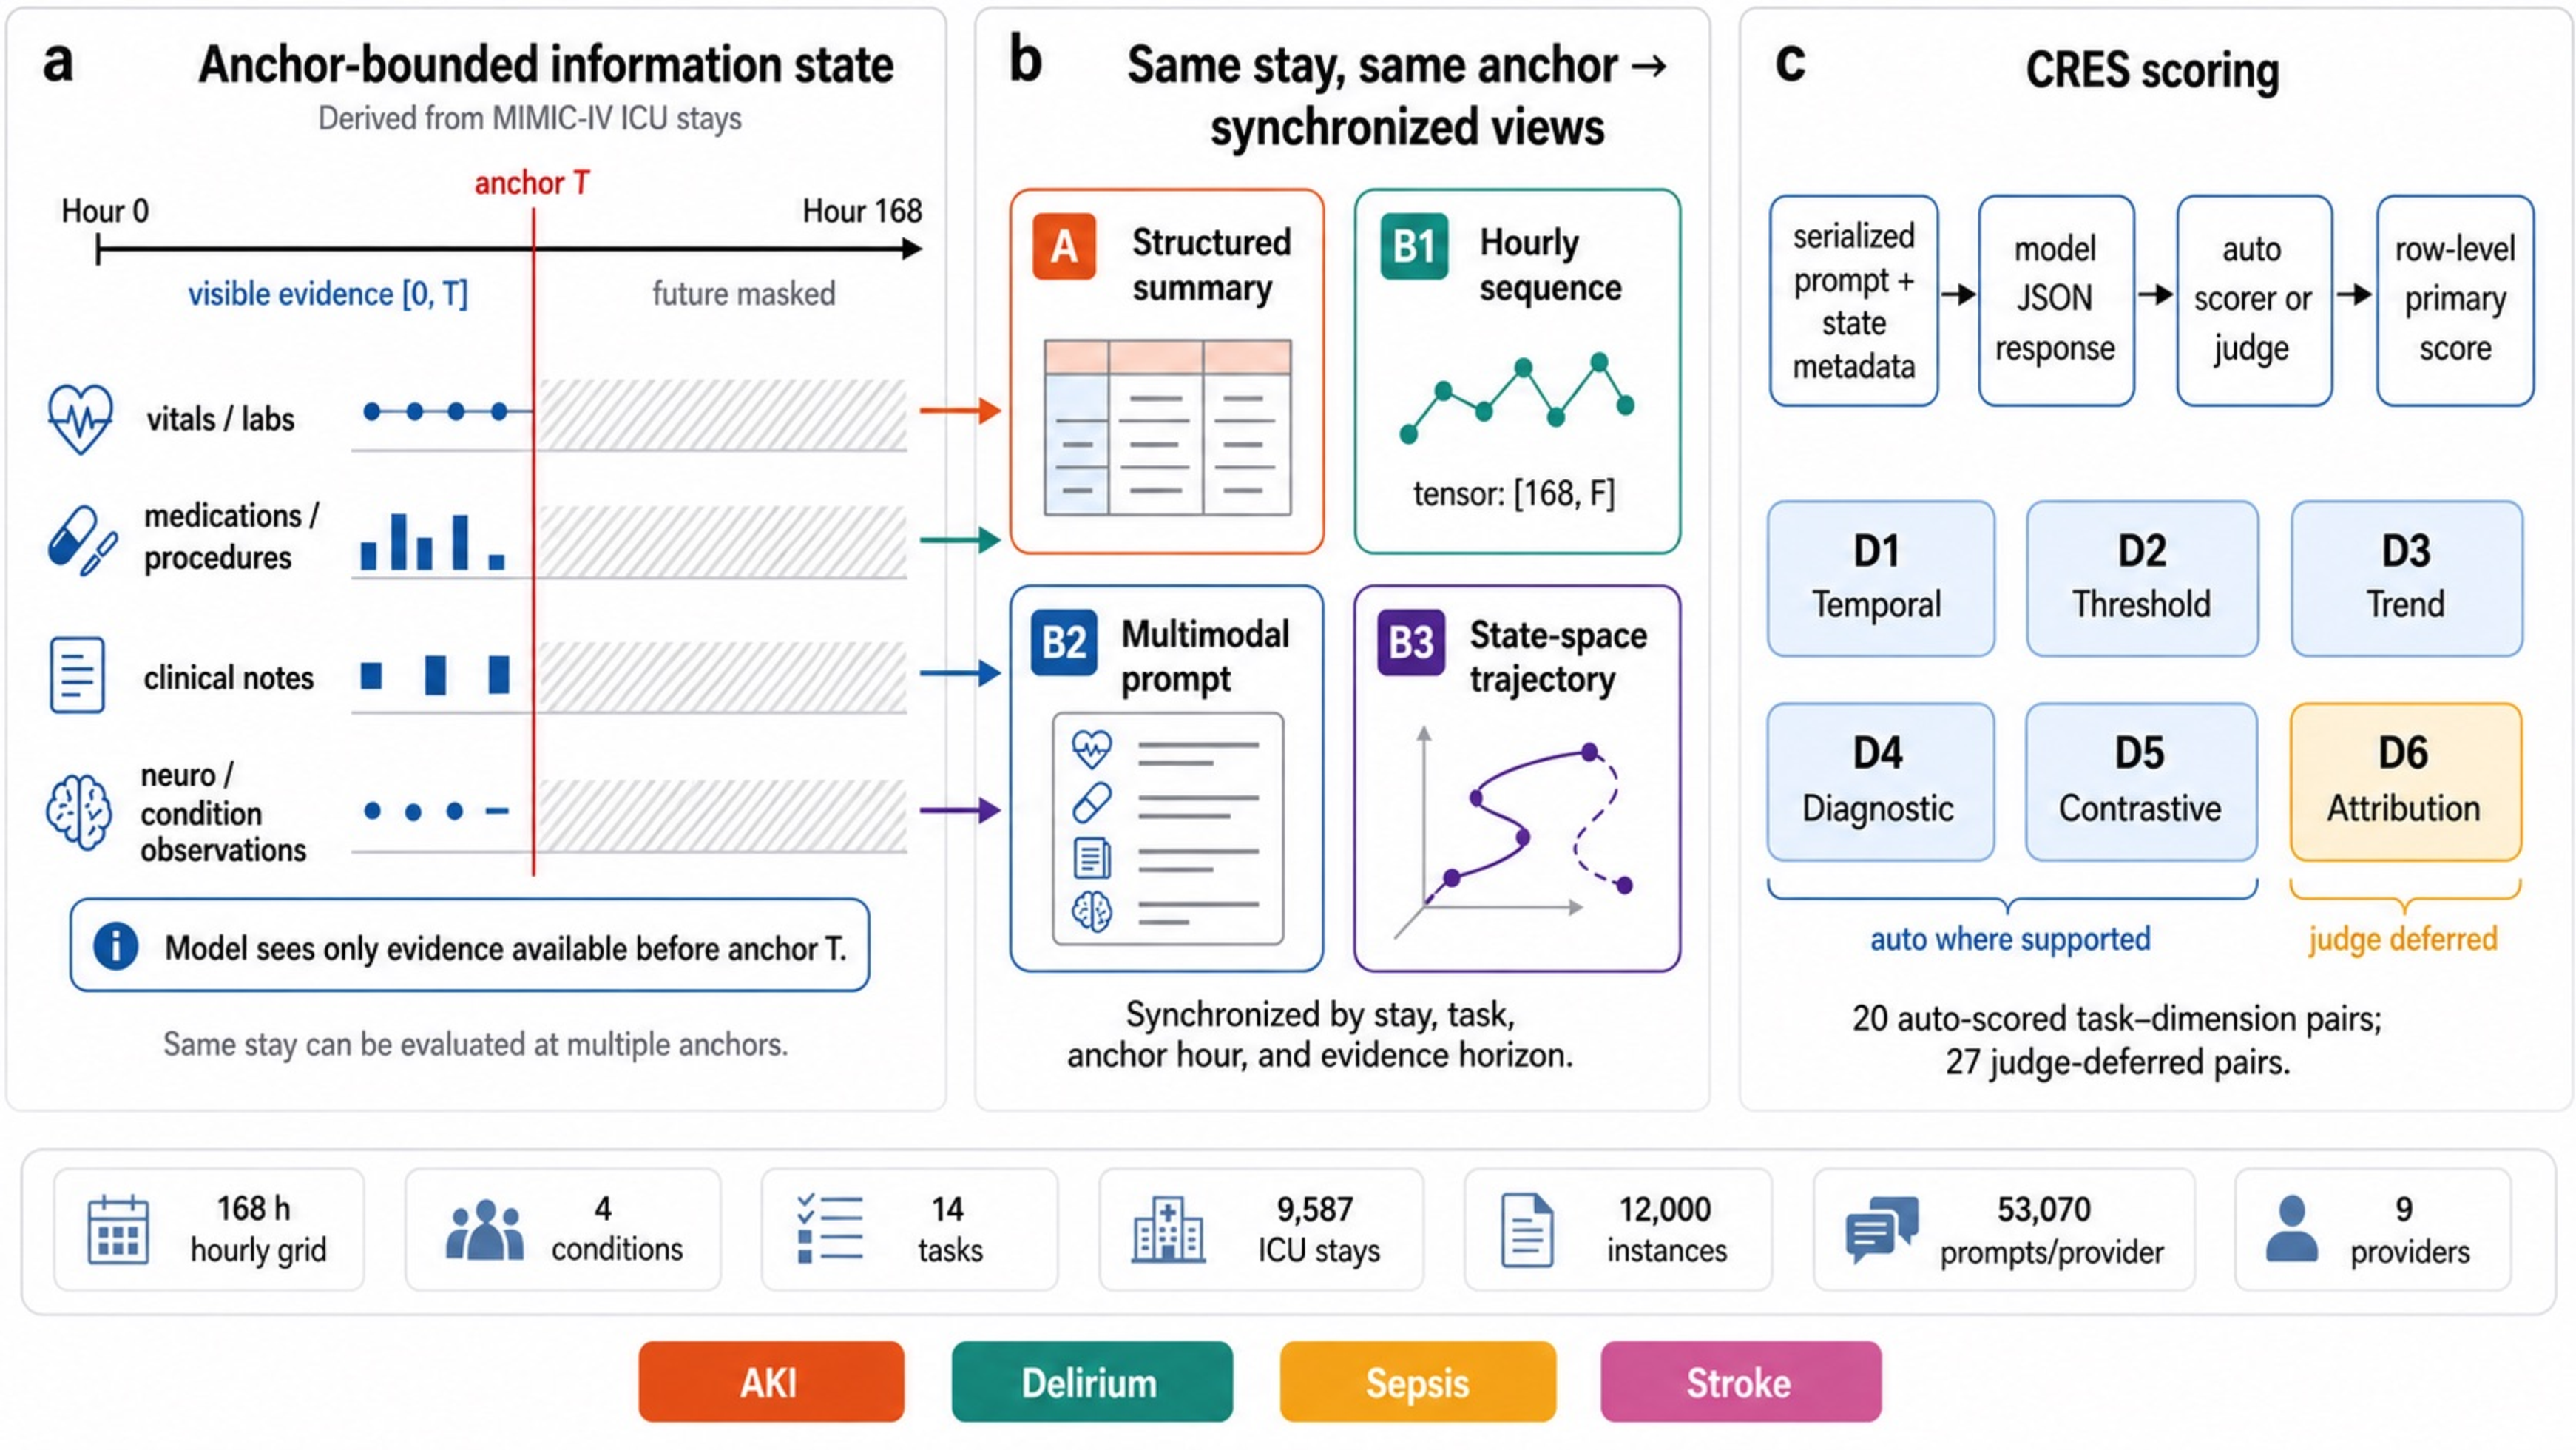
\includegraphics[width=\textwidth]{figures/main/figure1_information_state_anatomy.pdf}
\caption{TIMELY Bench evaluates temporal clinical reasoning by fixing the patient information state at an anchor hour and synchronizing multiple representations of the same ICU stay. Panel a shows that models can only use evidence visible in [0, T], with future information masked. Panel b shows the four synchronized benchmark views: Branch A structured summary, Branch B1 hourly sequence, Branch B2 multimodal EHR prompt, and Branch B3 state-space trajectory. Panel c shows how a Clinical Reasoning Evaluation Suite (CRES) instance maps a stay, task, dimension, and anchor into a serialized prompt, JSON response, and scorer. The bottom scale strip summarizes the frozen evaluation scale.}
\label{fig:architecture}
\end{figure*}

\FloatBarrier

\section{Results}

We report the benchmark in the same order as the three research questions. The first analyses compare explicit temporal structure with compact summaries and compare medical-domain models with general-purpose models. We then examine condition-level difficulty, temporal sensitivity, trajectory-template support, and judge-rated response quality.

\subsection{Dataset scale and benchmark composition}

TIMELY Bench is a multi-condition, multi-task benchmark, not a repeated binary prediction template. The full condition-level release covered 2,456,896 AKI task instances from 49,920 ICU stays, 1,512,502 delirium instances from 21,628 stays, 898,560 sepsis instances from 29,713 stays, and 61,111 stroke instances from 5,318 stays (Table~\ref{tab:dataset_condition}). AKI, delirium, and sepsis each contributed two onset- or state-oriented tasks on a common temporal scaffold. Stroke contributed eight tasks split across a Layer 1 temporal block and a Layer 2 retrospective or extraction block, reflecting a distinct reasoning regime.

Representation availability also differed by condition family. Branches A, B1, and B2 were available for all four conditions, whereas B3 and the downstream template-matching layer were only available for AKI, delirium, and sepsis. This asymmetry was deliberate. Stroke retained the same anchor-bounded multimodal design but was not forced into the physiology-template stack because its progression signals were organized around neurological deficit structure, laterality, imaging concordance, and retrospective discharge synthesis rather than around a single executable phase template.

Task-level class balance showed that the benchmark does not collapse to one generic difficulty setting (Table~\ref{tab:dataset_task}). Positive rates ranged from 0.98\% for AKI-S1 and 1.66\% for SEP-T1 to approximately 21--22\% for the delirium tasks. Stroke tasks combined binary, categorical, and numeric extraction settings. These differences matter because a benchmark can otherwise overstate generality while repeatedly measuring the same underlying behavior.

The frozen formal evaluation sample contained 12,000 benchmark instances from 9,587 unique ICU stays. Sampling was capped at two anchors per stay per task, with one early anchor at or before 12 hours and one late anchor at or after 24 hours, to reduce domination by a small number of long stays. Expanding these sampled instances across the supported task-dimension mapping yielded 53,070 \texttt{full\_multimodal} prompts per provider. All formal comparative and judge-facing analyses reported here use this frozen evaluation sample only.

Prompt length varied substantially across conditions. Using a conservative whitespace-based approximation to a \texttt{cl100k}-style tokenizer ($\times 1.3$), the median \texttt{full\_multimodal} prompt contained approximately 1,724 tokens (interquartile range 807--2,564; range 183--15,040), with a mean of 1,978 tokens. Stroke prompts were the longest on average (median 2,359 tokens), followed by delirium (1,999), AKI (1,580), and sepsis (1,120). At the task level, stroke retrospective task S-R4 had the longest median prompt length (4,007 tokens), whereas S-T2 was the shortest (334 tokens). Clinical notes contributed 58.7\% of prompt tokens on average, with the remainder distributed mainly across the structured timeline (15.7\%) and medication sections (14.8\%). These prompt lengths were compatible with the effective context windows of the frozen nine-provider comparative set after the pre-freeze contestant substitutions described in Methods.

\begin{table*}[t]
\caption{Dataset statistics. Panel A summarizes condition-level cohort size, task count, task roster, and representation availability.}
\label{tab:dataset_condition}
\centering
\scriptsize
\begin{tabularx}{\textwidth}{@{}lrr>{\raggedright\arraybackslash}X>{\raggedright\arraybackslash}Xc@{}}
\toprule
Condition & Instances & Unique stays & Tasks & Representations & B3 \\
\midrule
AKI & 2,456,896 & 49,920 & AKI-S1, AKI-T1 & A/B1/B2/B3 & yes \\
Delirium & 1,512,502 & 21,628 & DEL-S1, DEL-T1 & A/B1/B2/B3 & yes \\
Sepsis & 898,560 & 29,713 & SEP-S1, SEP-T1 & A/B1/B2/B3 & yes \\
Stroke & 61,111 & 5,318 & S-R1, S-R2, S-R3, S-R4, S-T1, S-T2, S-T3, S-T4 & A/B1/B2 & no \\
\botrule
\end{tabularx}
\normalsize
\end{table*}


\addtocounter{table}{-1}
\begingroup
\renewcommand{\theHtable}{table.panelb}
\scriptsize
\begin{longtable}{@{}ll>{\raggedright\arraybackslash}p{2.8cm}rr>{\raggedright\arraybackslash}p{1.8cm}>{\raggedright\arraybackslash}p{3.2cm}@{}}
\caption{Dataset statistics. Panel B summarizes task-level instance counts, unique stays, label summary, and representation availability. Disease prefixes denote AKI, delirium (DEL), sepsis (SEP), and stroke (S); task-family letters after the hyphen denote temporal or prospective tasks (T), secondary state or trajectory tasks (S), and retrospective stroke extraction or synthesis tasks (R).}\label{tab:dataset_task}\\
\toprule
Task & Condition & Layer / mode & Instances & Unique stays & Label summary & Representations \\
\midrule
\endfirsthead
\toprule
Task & Condition & Layer / mode & Instances & Unique stays & Label summary & Representations \\
\midrule
\endhead
AKI-S1 & AKI & single-layer temporal & 1,764,883 & 48,461 & 0.98\% & A/B1/B2/B3 \\
AKI-T1 & AKI & single-layer temporal & 692,013 & 40,915 & 8.46\% & A/B1/B2/B3 \\
DEL-S1 & Delirium & single-layer temporal & 756,251 & 21,628 & 22.03\% & A/B1/B2/B3 \\
DEL-T1 & Delirium & single-layer temporal & 756,251 & 21,628 & 21.10\% & A/B1/B2/B3 \\
SEP-S1 & Sepsis & single-layer temporal & 27,003 & 11,715 & 21.11\% & A/B1/B2/B3 \\
SEP-T1 & Sepsis & single-layer temporal & 871,557 & 26,517 & 1.66\% & A/B1/B2/B3 \\
S-R1 & Stroke & Layer 2 retrospective & 3,912 & 3,912 & 5 classes & B2 \\
S-R2 & Stroke & Layer 2 retrospective & 3,912 & 3,912 & 4 classes & B2 \\
S-R3 & Stroke & Layer 2 retrospective & 277 & 277 & median=2.5 & B2 \\
S-R4 & Stroke & Layer 2 retrospective & 3,912 & 3,912 & 8.79\% & B2 \\
S-T1 & Stroke & Layer 1 temporal & 36,519 & 4,792 & 14.25\% & A/B1/B2 \\
S-T2 & Stroke & Layer 1 temporal & 4,952 & 4,952 & 5 classes & A/B1/B2 \\
S-T3 & Stroke & Layer 1 temporal & 2,651 & 2,651 & 3 classes & A/B1/B2 \\
S-T4 & Stroke & Layer 1 temporal & 4,976 & 4,976 & 16 classes & A/B1/B2 \\
\botrule
\end{longtable}
\normalsize

\endgroup

\FloatBarrier

\subsection{Explicit temporal structure helped selectively}

The branch comparison tested RQ1 by asking whether the hourly sequence improves performance over a compact anchor-state summary.

Structured baselines were strong on several tasks and provided an important anchor for interpreting the LLM results. Branch A XGBoost reached AUROC 0.977 for AKI-S1, 0.941 for AKI-T1, 0.918 and 0.916 for the two delirium tasks, and 0.950 for SEP-T1 (Table~\ref{tab:structured_baselines}). The same branch was materially weaker on SEP-S1 (AUROC 0.751) and S-T1 (AUROC 0.726), consistent with the idea that these tasks require more than stable tabular summarization.

The key branch comparison finding is that an explicit hourly sequence did not uniformly dominate a compact summary representation. Using the B1 model selected by AUROC for each task as the shared B1 comparator, B1 improved AUROC on only three of seven eligible tasks: AKI-S1, AKI-T1, and SEP-T1. Using the same AUROC-selected B1 comparator, it improved AUPRC on only one task, AKI-T1. The clearest B1 gain was AKI-T1, where BiLSTM-attention improved AUROC from 0.941 to 0.949 and AUPRC from 0.595 to 0.603. The clearest B1 deficit was SEP-S1, where the AUROC-selected B1 model underperformed A by 0.047 AUROC and 0.057 AUPRC.

This pattern argues against a simple ``more temporal detail is always better'' interpretation. Explicit temporal structure helped when the target depended on an evolving trajectory that the summary representation compressed away. It did not help when the sequence mainly added noise or when the anchor-state summary already captured the decision signal. That distinction is central to TIMELY Bench's purpose: it measures when temporal structure is informative, not just whether it can be preserved.

\begin{table*}[t]
\caption{Structured baselines on eligible binary tasks. Five-fold subject-level cross-validation results for Branch A and Branch B1, reported as mean AUROC and AUPRC.}
\label{tab:structured_baselines}
\centering
\scriptsize
\begin{tabular}{@{}llllrr@{}}
\toprule
Task & Condition & Branch & Model & AUROC & AUPRC \\
\midrule
AKI-S1 & AKI & A & xgboost & 0.977 & 0.372 \\
AKI-S1 & AKI & B1 & temporal\_transformer & 0.978 & 0.346 \\
AKI-S1 & AKI & B1 & bilstm\_attention & 0.977 & 0.339 \\
AKI-T1 & AKI & A & xgboost & 0.941 & 0.595 \\
AKI-T1 & AKI & B1 & bilstm\_attention & 0.949 & 0.603 \\
AKI-T1 & AKI & B1 & temporal\_transformer & 0.941 & 0.562 \\
DEL-S1 & Delirium & A & xgboost & 0.918 & 0.702 \\
DEL-S1 & Delirium & B1 & temporal\_transformer & 0.911 & 0.689 \\
DEL-S1 & Delirium & B1 & bilstm\_attention & 0.910 & 0.702 \\
DEL-T1 & Delirium & A & xgboost & 0.916 & 0.692 \\
DEL-T1 & Delirium & B1 & bilstm\_attention & 0.908 & 0.659 \\
DEL-T1 & Delirium & B1 & temporal\_transformer & 0.894 & 0.615 \\
SEP-S1 & Sepsis & A & xgboost & 0.751 & 0.465 \\
SEP-S1 & Sepsis & B1 & bilstm\_attention & 0.704 & 0.408 \\
SEP-S1 & Sepsis & B1 & temporal\_transformer & 0.643 & 0.338 \\
SEP-T1 & Sepsis & A & xgboost & 0.950 & 0.329 \\
SEP-T1 & Sepsis & B1 & bilstm\_attention & 0.953 & 0.275 \\
SEP-T1 & Sepsis & B1 & temporal\_transformer & 0.948 & 0.258 \\
S-T1 & Stroke & A & xgboost & 0.726 & 0.251 \\
S-T1 & Stroke & B1 & bilstm\_attention & 0.707 & 0.247 \\
S-T1 & Stroke & B1 & temporal\_transformer & 0.676 & 0.230 \\
\botrule
\end{tabular}
\normalsize
\end{table*}


\begin{figure*}[t]
\centering
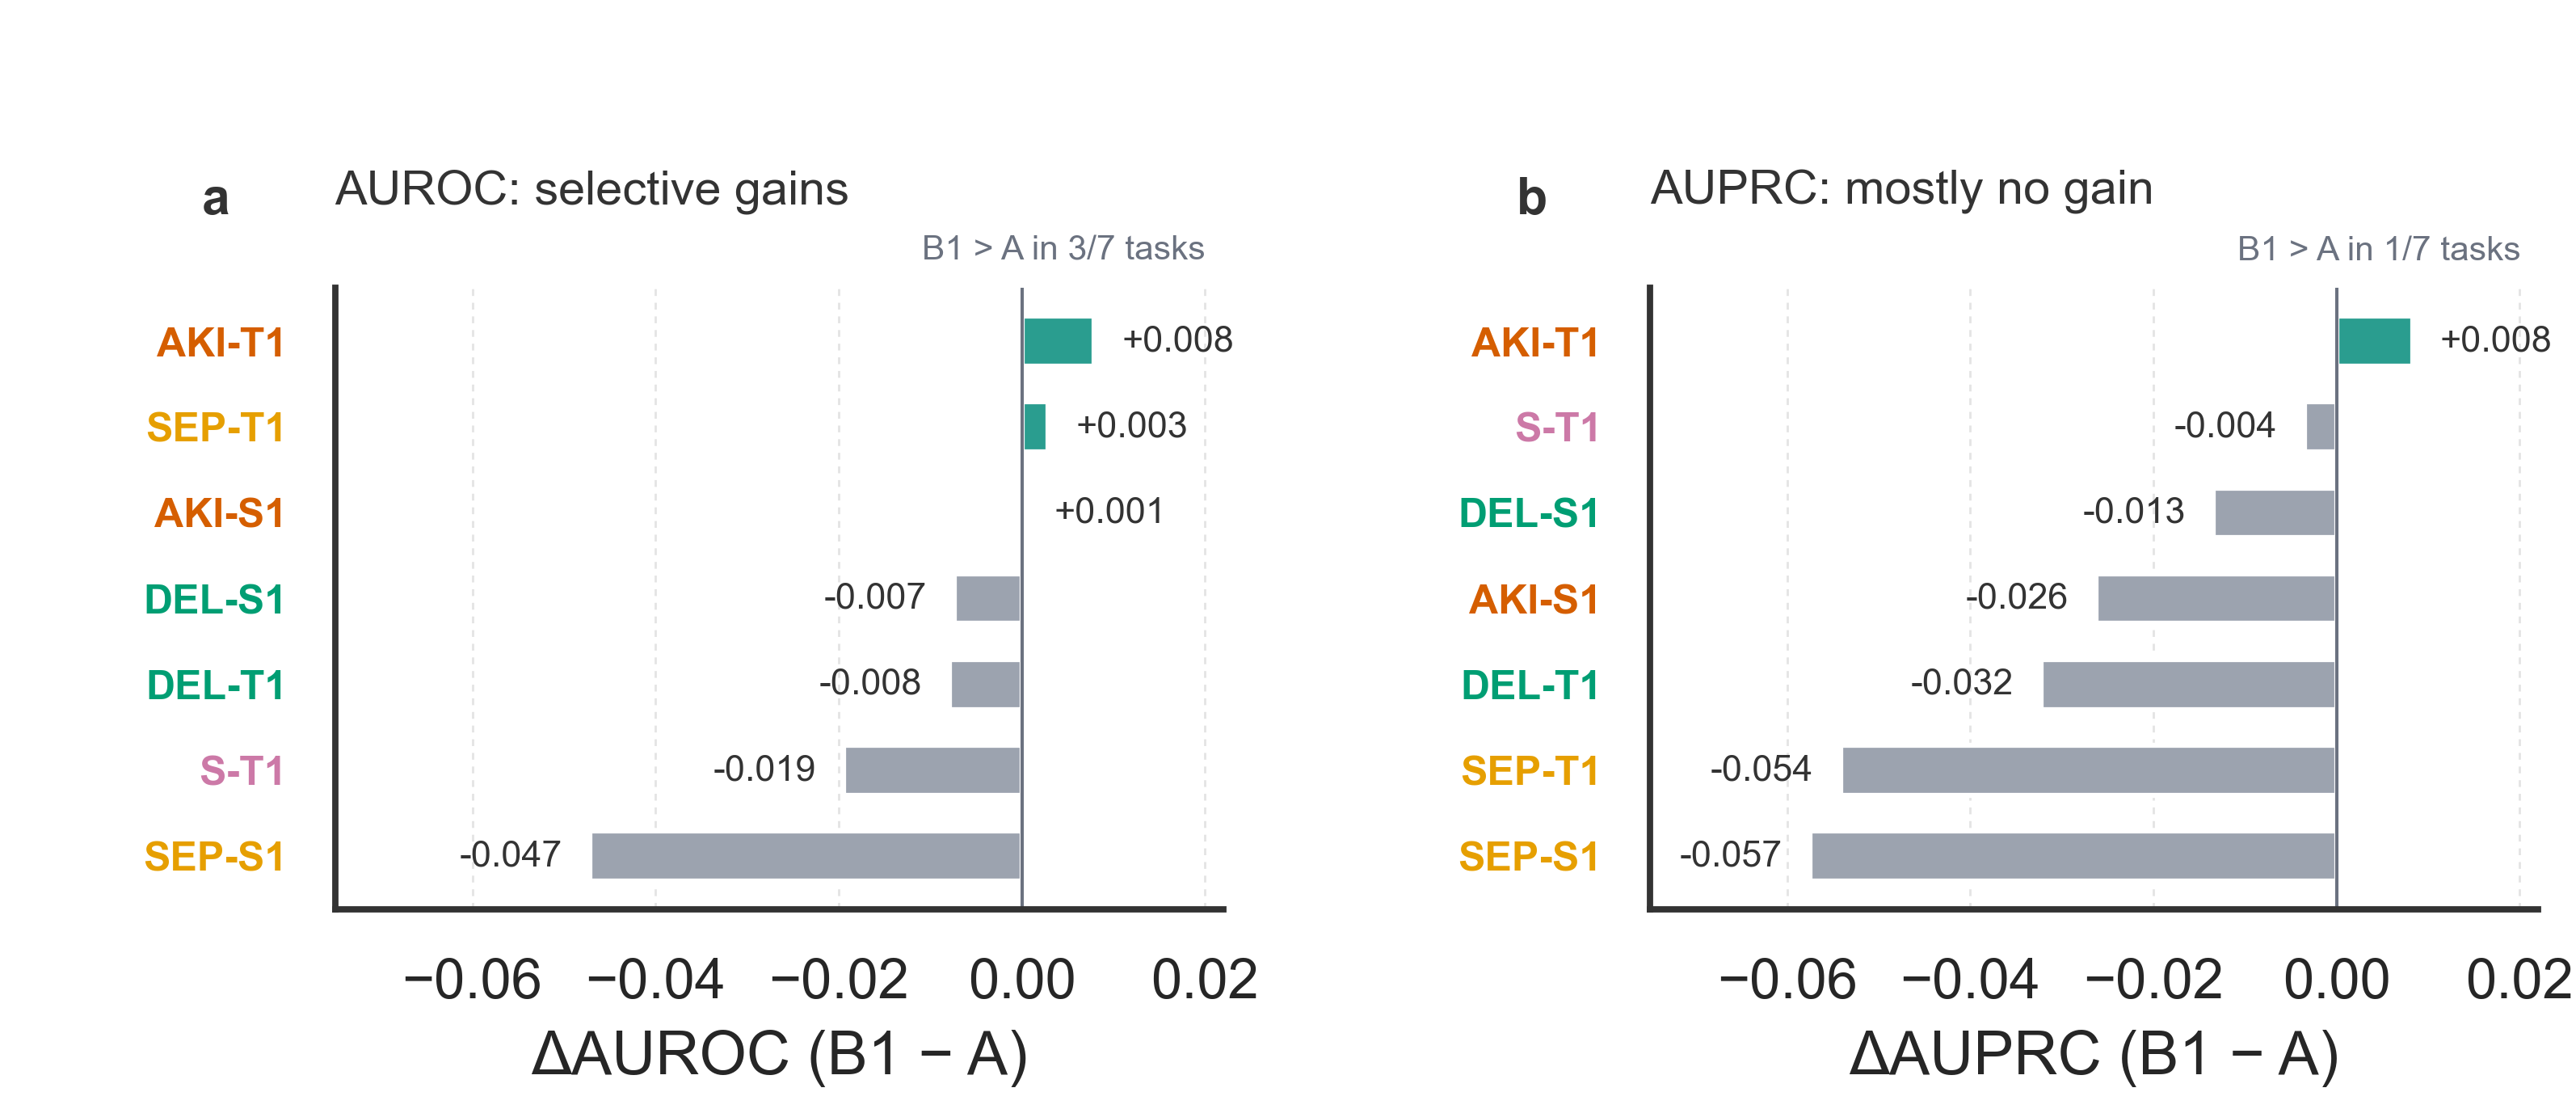
\includegraphics[width=\textwidth]{figures/main/figure2_branch_delta_first.png}
\caption{Explicit hourly sequence modeling improved performance only selectively, indicating that the value of temporal detail was task-dependent. Panel a shows delta AUROC and panel b shows delta AUPRC, both computed as Branch B1 minus Branch A for the seven eligible binary tasks. For each task, Branch B1 is represented by the B1 model selected by AUROC, and both AUROC and AUPRC deltas are computed using that same selected B1 comparator relative to Branch A. B1 improved AUROC in 3/7 tasks (AKI-S1, AKI-T1, SEP-T1) and improved AUPRC in 1/7 tasks (AKI-T1 only). Negative deltas indicate tasks where the simpler structured baseline outperformed the explicit hourly-sequence model.}
\label{fig:branch_comparison}
\end{figure*}

\FloatBarrier

\subsection{General-purpose models led the aggregate ranking}

The provider comparison tested RQ3 by evaluating whether medical-domain adaptation improved anchor-bounded temporal reasoning over synchronized ICU evidence.

Formal cross-provider comparison covered nine frozen providers: two Tier 1A closed general-purpose API models, three Tier 1B general-purpose open or semi-open models, and four Tier 2 medical-domain adapted models. Tier labels were analysis strata rather than performance-derived categories. Macro primary score is a provider's equal-weight mean over the 20 supported task-dimension primary scores, not a row-weighted average. Overall macro primary score ranged from 0.489 to 0.655 (Table~\ref{tab:provider_ranking}). The overall leader was Gemini 3.1 Pro at 0.655, followed by Gemma4-26B at 0.646, DeepSeek Chat at 0.635, and Qwen3.5 at 0.634. GPT-5.4 ranked fifth overall at 0.626 despite leading the AKI condition family.

The tier pattern was the more clinically relevant result. The best Tier 2 model, MedGemma-4B, reached a macro primary score of 0.535, below all Tier 1A and Tier 1B providers. Aloe-70B, Meditron3-8B, and Aloe-7B followed at 0.519, 0.510, and 0.489. Current medical-domain adaptation did not translate into superior temporal multimodal reasoning on this benchmark. The gap was not driven by one isolated condition.

Condition-level summaries clarify why overall averages should be interpreted cautiously (Table~\ref{tab:condition_summary}; Fig.~\ref{fig:provider_comparison}). Delirium was near ceiling for several providers. AKI strongly favored GPT-5.4 and Gemini 3.1 Pro. Sepsis favored Tier 1B models such as Gemma4-26B and Qwen3.5. Stroke remained difficult for all tiers, with condition-level macro scores far below those of the other three families. These differences are not noise around one latent capability axis; they indicate that temporal clinical reasoning difficulty is condition-specific.

\begin{table*}[t]
\caption{Frozen cross-provider comparative ranking across the nine-provider formal comparative set. Pair wins denote the number of supported task-dimension pairs for which the provider achieved the highest primary score within its tier; ties are counted for all co-winning providers.}
\label{tab:provider_ranking}
\centering
\scriptsize
\begin{tabular}{@{}llrrrr@{}}
\toprule
Provider & Tier & Macro score & Pair wins & Avg latency (s) & Total tokens \\
\midrule
Gemini 3.1 Pro & Tier 1A & 0.655 & 16 & 15.938 & 343,643,633 \\
Gemma4-26B & Tier 1B & 0.646 & 12 & 30.038 & 277,833,535 \\
DeepSeek Chat & Tier 1B & 0.635 & 10 & 12.711 & 261,196,668 \\
Qwen3.5 & Tier 1B & 0.634 & 4 & 4.843 & 285,969,716 \\
GPT-5.4 & Tier 1A & 0.626 & 9 & 11.401 & 264,064,840 \\
MedGemma-4B & Tier 2 & 0.535 & 8 & 71.572 & 285,394,344 \\
Aloe-70B & Tier 2 & 0.519 & 11 & 5.710 & 258,039,766 \\
Meditron3-8B & Tier 2 & 0.510 & 7 & 3.198 & 259,948,539 \\
Aloe-7B & Tier 2 & 0.489 & 7 & 2.759 & 282,111,131 \\
\botrule
\end{tabular}
\normalsize
\end{table*}


\scriptsize
\begin{longtable}{@{}llllr@{}}
\caption{Condition-level comparative summary. Condition-stratified provider performance summarized as macro primary score within each condition family.}\label{tab:condition_summary}\\
\toprule
Provider & Tier & Condition & Macro score & Pairs \\
\midrule
\endfirsthead
\toprule
Provider & Tier & Condition & Macro score & Pairs \\
\midrule
\endhead
GPT-5.4 & Tier 1A & AKI & 0.789 & 5 \\
Gemini 3.1 Pro & Tier 1A & AKI & 0.786 & 5 \\
DeepSeek Chat & Tier 1B & AKI & 0.753 & 5 \\
Gemma4-26B & Tier 1B & AKI & 0.708 & 5 \\
Qwen3.5 & Tier 1B & AKI & 0.679 & 5 \\
MedGemma-4B & Tier 2 & AKI & 0.477 & 5 \\
Aloe-70B & Tier 2 & AKI & 0.458 & 5 \\
Meditron3-8B & Tier 2 & AKI & 0.418 & 5 \\
Aloe-7B & Tier 2 & AKI & 0.342 & 5 \\
DeepSeek Chat & Tier 1B & Delirium & 1.000 & 3 \\
Gemini 3.1 Pro & Tier 1A & Delirium & 1.000 & 3 \\
GPT-5.4 & Tier 1A & Delirium & 1.000 & 3 \\
Aloe-70B & Tier 2 & Delirium & 1.000 & 3 \\
Gemma4-26B & Tier 1B & Delirium & 0.996 & 3 \\
Qwen3.5 & Tier 1B & Delirium & 0.993 & 3 \\
Aloe-7B & Tier 2 & Delirium & 0.964 & 3 \\
Meditron3-8B & Tier 2 & Delirium & 0.958 & 3 \\
MedGemma-4B & Tier 2 & Delirium & 0.883 & 3 \\
Gemma4-26B & Tier 1B & Sepsis & 0.833 & 4 \\
Qwen3.5 & Tier 1B & Sepsis & 0.822 & 4 \\
Gemini 3.1 Pro & Tier 1A & Sepsis & 0.802 & 4 \\
DeepSeek Chat & Tier 1B & Sepsis & 0.795 & 4 \\
GPT-5.4 & Tier 1A & Sepsis & 0.750 & 4 \\
MedGemma-4B & Tier 2 & Sepsis & 0.714 & 4 \\
Meditron3-8B & Tier 2 & Sepsis & 0.686 & 4 \\
Aloe-7B & Tier 2 & Sepsis & 0.632 & 4 \\
Aloe-70B & Tier 2 & Sepsis & 0.556 & 4 \\
Gemma4-26B & Tier 1B & Stroke & 0.382 & 8 \\
Qwen3.5 & Tier 1B & Stroke & 0.376 & 8 \\
Gemini 3.1 Pro & Tier 1A & Stroke & 0.371 & 8 \\
Aloe-70B & Tier 2 & Stroke & 0.359 & 8 \\
MedGemma-4B & Tier 2 & Stroke & 0.350 & 8 \\
DeepSeek Chat & Tier 1B & Stroke & 0.344 & 8 \\
Aloe-7B & Tier 2 & Stroke & 0.331 & 8 \\
GPT-5.4 & Tier 1A & Stroke & 0.321 & 8 \\
Meditron3-8B & Tier 2 & Stroke & 0.312 & 8 \\
\botrule
\end{longtable}
\normalsize


\begin{figure*}[t]
\centering
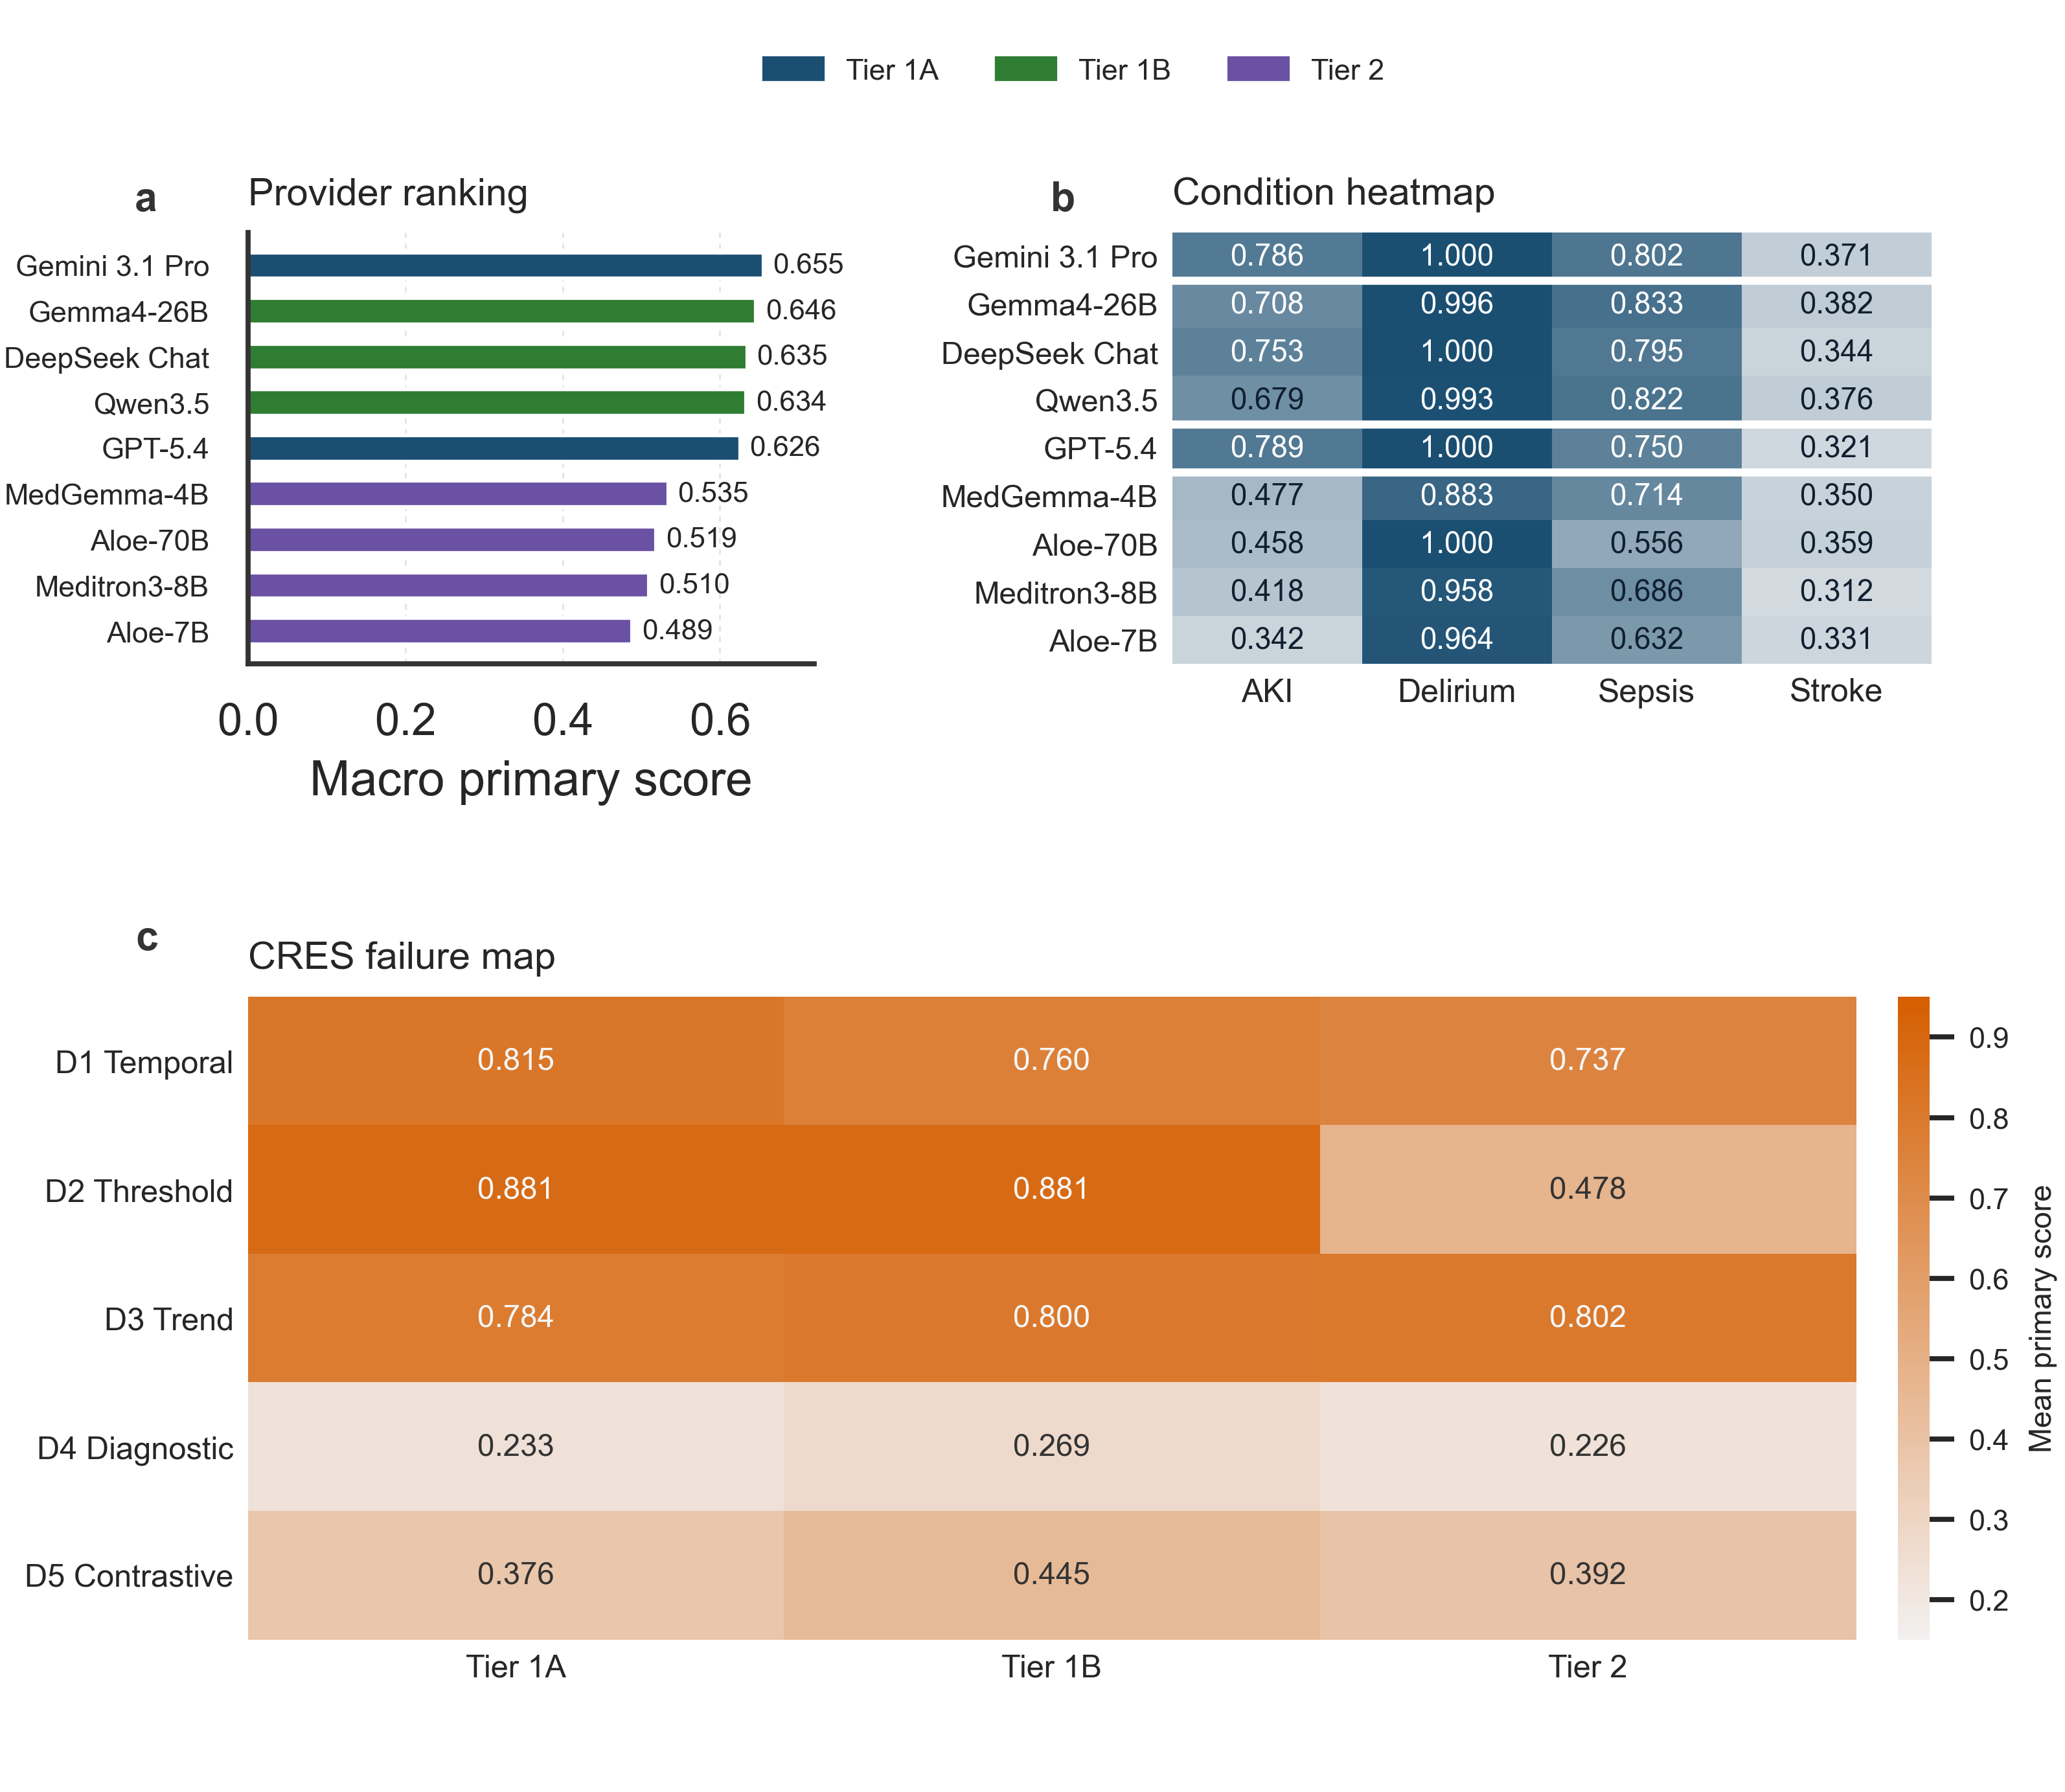
\includegraphics[width=\textwidth]{figures/main/figure3_provider_condition_cres.png}
\caption{General-purpose models led the frozen comparison, while Clinical Reasoning Evaluation Suite (CRES) stratification showed dimension-specific failure patterns. Panel a shows overall macro primary score by provider, with bars colored by model tier. Panel b shows condition-level macro primary scores across AKI, delirium, sepsis, and stroke. Panel c shows mean primary score by CRES dimension and provider tier for auto-scored dimensions D1--D5. D1--D5 are auto-scored where supported; D6 attribution is judge-deferred and excluded from primary auto-scoring.}
\label{fig:provider_comparison}
\end{figure*}

\FloatBarrier

\subsection{Per-dimension CRES analysis exposed distinct reasoning failure modes}

The CRES dimension analysis separated overall accuracy into the reasoning operations that produced the condition and tier differences. CRES treats each prompt as testing one clinically interpretable operation rather than one undifferentiated accuracy score.

TIMELY Bench evaluates reasoning dimensions as well as task-level macro performance; operational definitions for D1--D6 are provided in Table~\ref{tab:cres_dimensions} in Methods. Formal auto-scoring covered 20 supported task-dimension pairs. Twenty-seven pairs remained deferred, and D6 attribution was intentionally kept out of the primary auto-scored result set. The main auto-scoring analysis covers D1--D5 only, with D6 deferred to judge evaluation and qualitative inspection.

Across providers, D3 trend reasoning was the strongest auto-scored dimension (mean primary score 0.797), followed by D1 temporal localization (0.762) and D2 threshold reasoning (0.702). D5 contrastive reasoning was substantially lower (0.406), and D4 diagnostic discrimination was the weakest dimension overall (0.242). This ordering is clinically plausible. Trend classification over overt stroke motor trajectories is comparatively easy once the affected side is visible. Diagnostic discrimination requires choosing between mechanistic or consistency explanations and is far more brittle under sparse or partially contradictory evidence.

Tier-level differences were most striking for D2. Tier 1A and Tier 1B both averaged approximately 0.881 on threshold reasoning, whereas Tier 2 dropped to 0.478. This separation did not reflect uniform weakness in Tier 2 models; the same group performed competitively on D3 trend reasoning (0.802) and somewhat better on D5 than the Tier 1A group. Current medical fine-tuning appears especially weak when the task requires explicit threshold grounding to guideline-like criteria, such as KDIGO stage crossing or septic shock thresholds.

Condition-specific dimension behavior further clarifies the benchmark construct. D1 temporal localization was essentially near ceiling for delirium (0.9999) and sepsis (0.9960), moderate for AKI (0.6509), and near floor for stroke (0.0399). D2 threshold reasoning was similarly high for delirium (0.9317), intermediate for stroke (0.7500) and AKI (0.6535), and markedly lower for sepsis (0.5208), where the target depends on jointly interpreting MAP, vasopressor exposure, lactate availability, and onset chronology. The dimension mapping is intentionally task-specific, so these averages should not be read as interchangeable latent skills. D3 and D4 are driven largely by stroke tasks, while D5 is concentrated in AKI and sepsis contrastive prompts. The per-dimension results add interpretability to the condition-level summaries; they do not replace them.

\subsection{Confidence behavior varied independently of raw accuracy}

Confidence outputs provided a deployment-facing check on RQ3: whether high-scoring models also used uncertainty labels selectively.

Confidence behavior separated providers in a way that the primary score alone would miss. GPT-5.4 marked 37,086 of 53,070 outputs as \texttt{high} confidence, or 69.9\%. Gemini 3.1 Pro marked 52,635 of 53,070 outputs as \texttt{high}, or 99.2\%. DeepSeek Chat was closer to GPT-5.4 at 71.6\%, whereas Qwen3.5 and Gemma4-26B were also highly concentrated in the \texttt{high} category at 90.7\% and 94.9\%, respectively.

Gemini 3.1 Pro was the overall top provider by macro primary score, yet its confidence distribution was far more compressed than that of GPT-5.4. The benchmark separates correctness from selective use of the self-reported confidence field. In practical terms, a model that answers well but declares nearly everything \texttt{high} confidence leaves less room for downstream workflow triage, uncertainty-aware escalation, or selective abstention. TIMELY Bench's confidence field was included to make this behavior visible.

The pattern was therefore not confined to one provider family. High-performing models differed not only in correctness but also in how much information their confidence labels carried. TIMELY Bench exposes confidence compression as a recurring failure mode in high-performing LLMs, particularly when the output schema forces a coarse confidence vocabulary.

\subsection{Temporal sensitivity varied by condition}

The temporal stress test examined whether condition difficulty changed across early, middle, and later anchor windows.

Temporal degradation analysis used predefined anchor buckets instead of exact single-hour points: T6 for anchor hours 4--8, T24 for hours 18--30, and T48 for hours 46--50. Any provider-task-bucket cell with fewer than 25 instances was marked as insufficient support and excluded from the main plot. Delirium and stroke do not show a T24 marker in the main figure because the middle bucket failed the support threshold, not because the data were missing.

The temporal pattern was not monotonic (Fig.~\ref{fig:temporal_degradation}). Sepsis displayed a T24 peak before declining again at T48. A plausible explanation is signal concentration: the T24 window disproportionately captures high-information segments around sepsis-to-shock evolution, whereas T48 includes more heterogeneous and partially stabilized stays. The result is more specific than ``earlier is harder'' or ``later is easier.'' Anchor sensitivity depends on where clinically informative signal is concentrated along the trajectory.

\begin{figure*}[t]
\centering
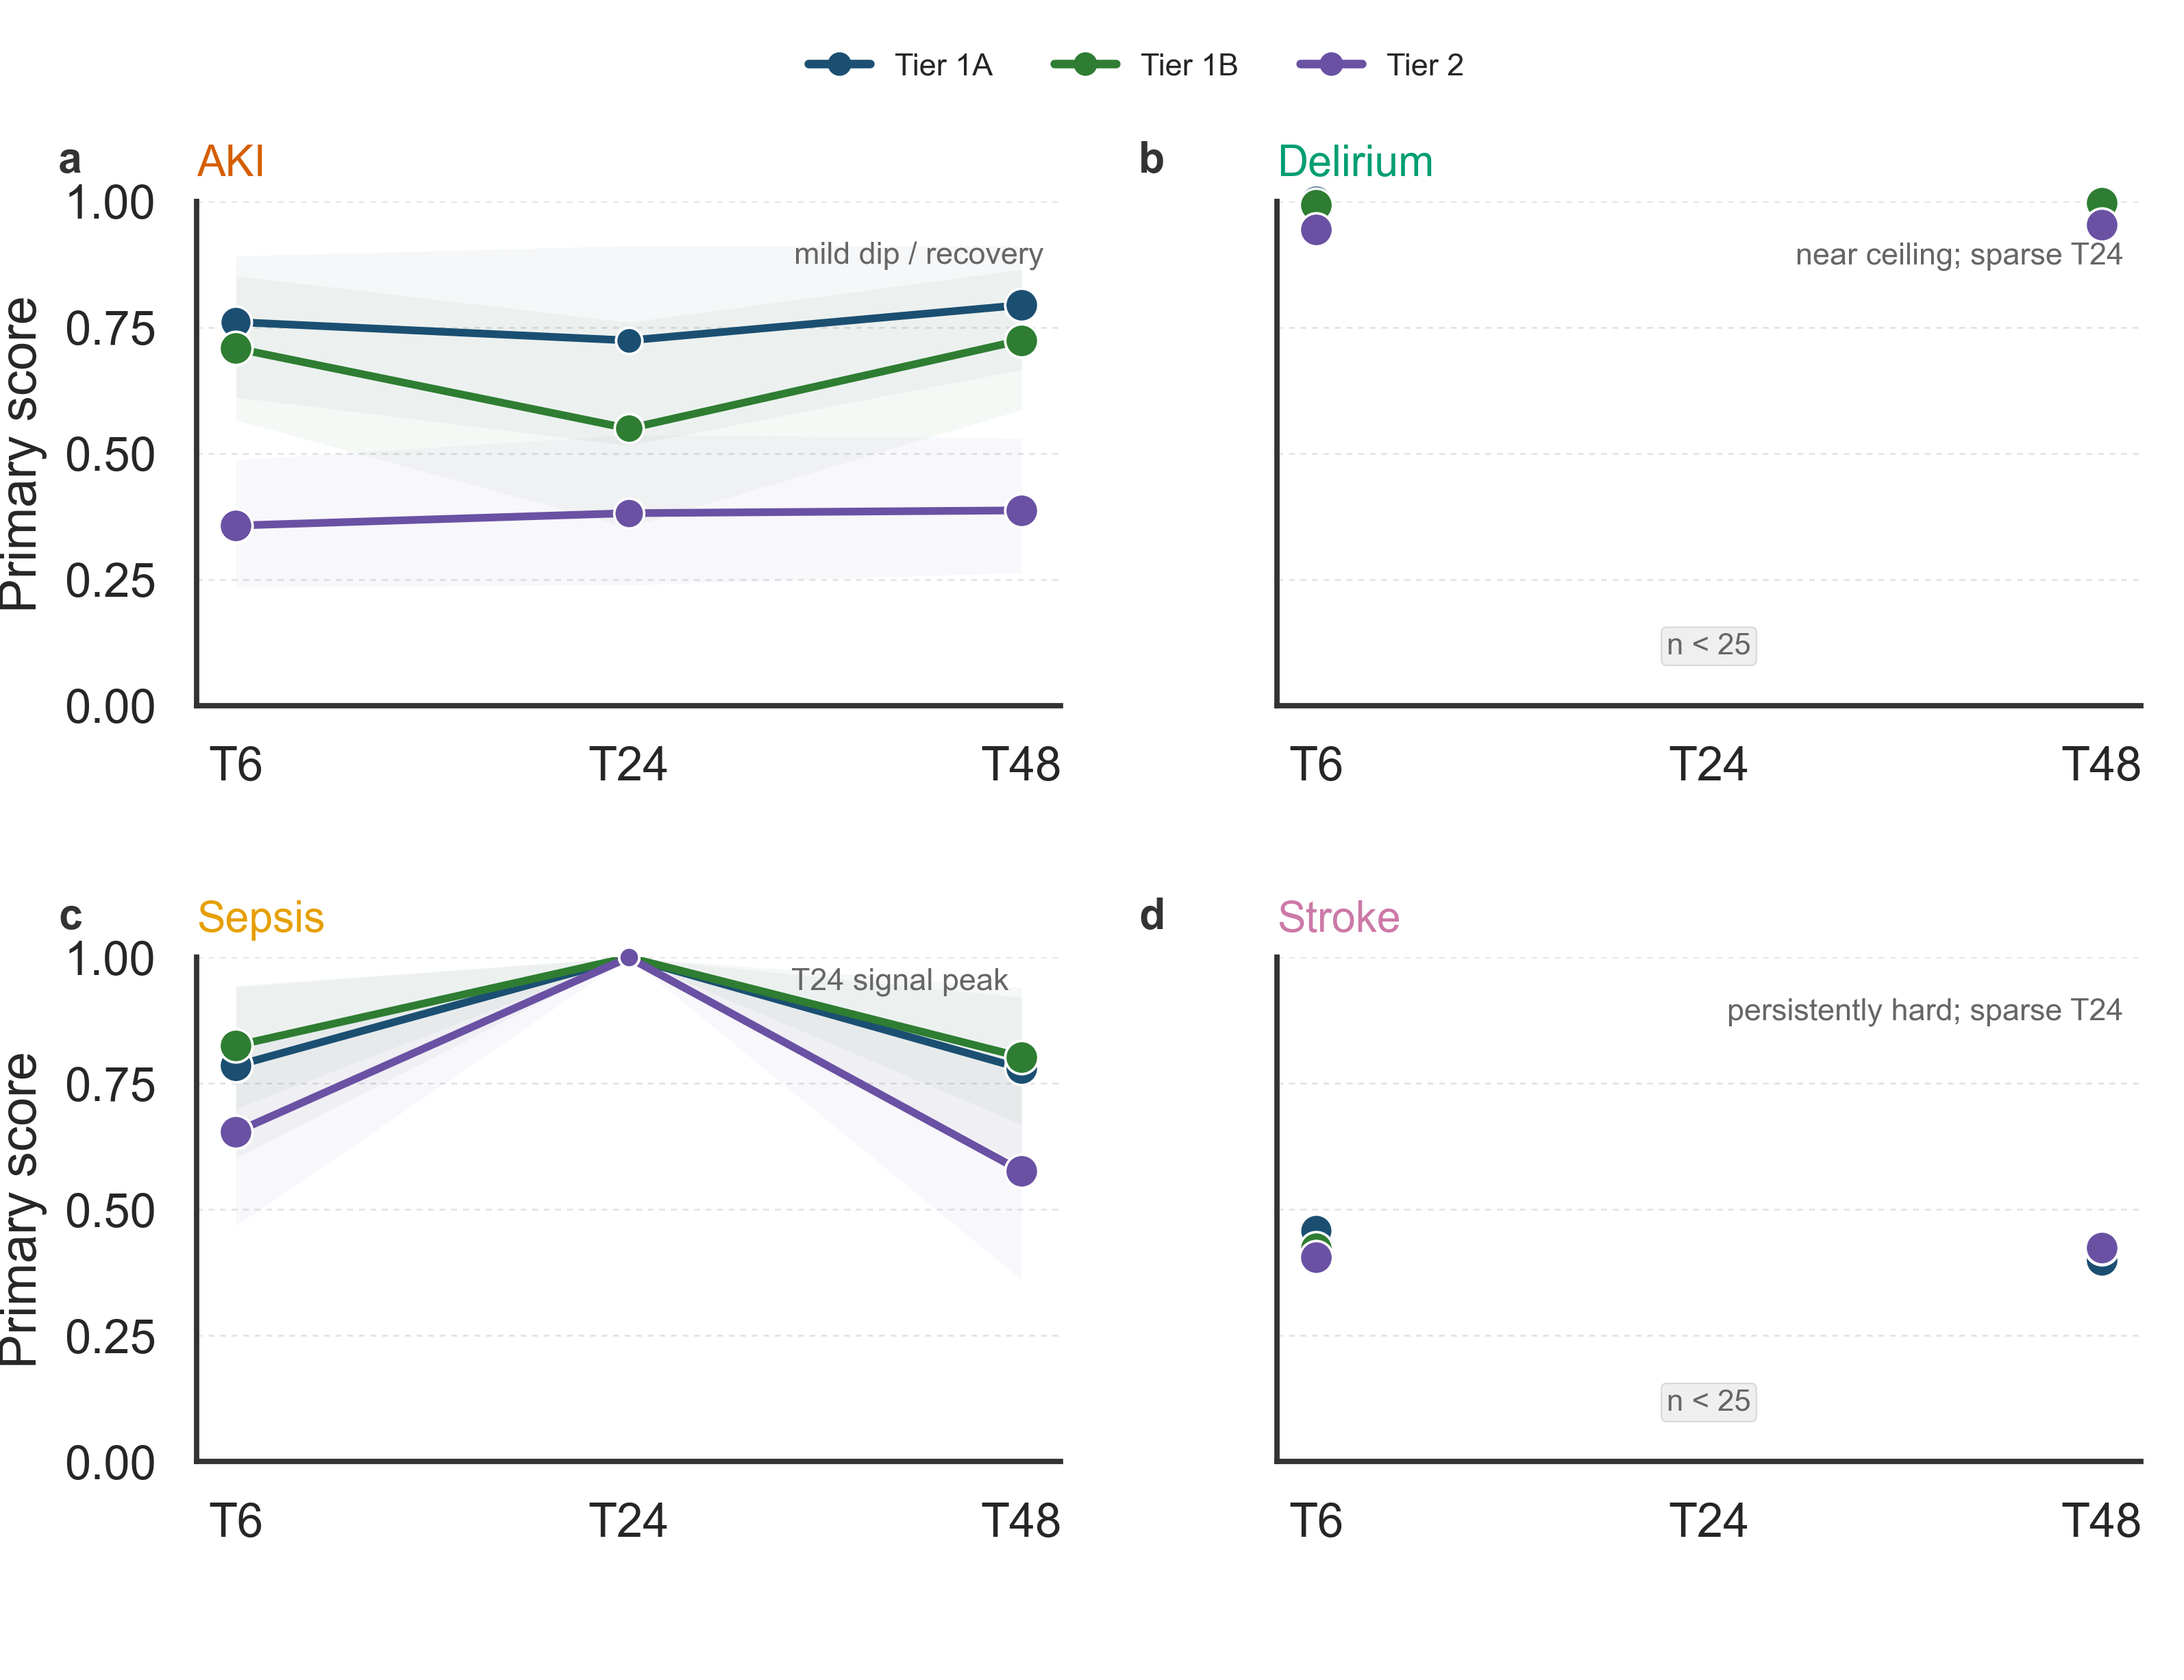
\includegraphics[width=\textwidth]{figures/main/figure4_temporal_stress_test.png}
\caption{Temporal sensitivity varied by condition and was not uniformly monotonic. Mean primary score is shown across predefined temporal buckets T6 (anchor hours 4--8), T24 (18--30), and T48 (46--50), stratified by provider tier and condition. Point size reflects the number of scored instances in each tier-condition-bucket cell, and shaded bands indicate bootstrap uncertainty where available. Cells with fewer than 25 instances were marked as insufficient support rather than treated as missing data. Sepsis showed a T24 signal peak, whereas delirium remained near ceiling and stroke remained persistently difficult.}
\label{fig:temporal_degradation}
\end{figure*}

\FloatBarrier

\subsection{The stroke two-layer split captured a real reasoning boundary}

The stroke analysis separated prospective temporal prediction from retrospective synthesis within the same condition family.

Stroke was designed differently from the other three conditions because it contains two qualitatively distinct reasoning regimes. Layer 1 evaluates anchor-bounded temporal prediction over evolving neurological observations. Layer 2 evaluates retrospective mechanism, strategy, numeric extraction, and complication reasoning using discharge and stay-level context. The empirical results support this split.

Layer 2 outperformed Layer 1 for all nine providers, with a mean Layer 2 minus Layer 1 gain of 0.130 macro primary score (Fig.~\ref{fig:stroke_layers}). The largest gains were observed for MedGemma-4B (+0.240), Gemma4-26B (+0.168), and Aloe-7B (+0.167). Retrospective synthesis from the full documented course was easier than short-horizon temporal stroke prediction under anchor masking. The same clinical story becomes much harder when the model must judge deterioration from partial evolving evidence, which is why stroke was separated into two layers.

\begin{figure*}[t]
\centering
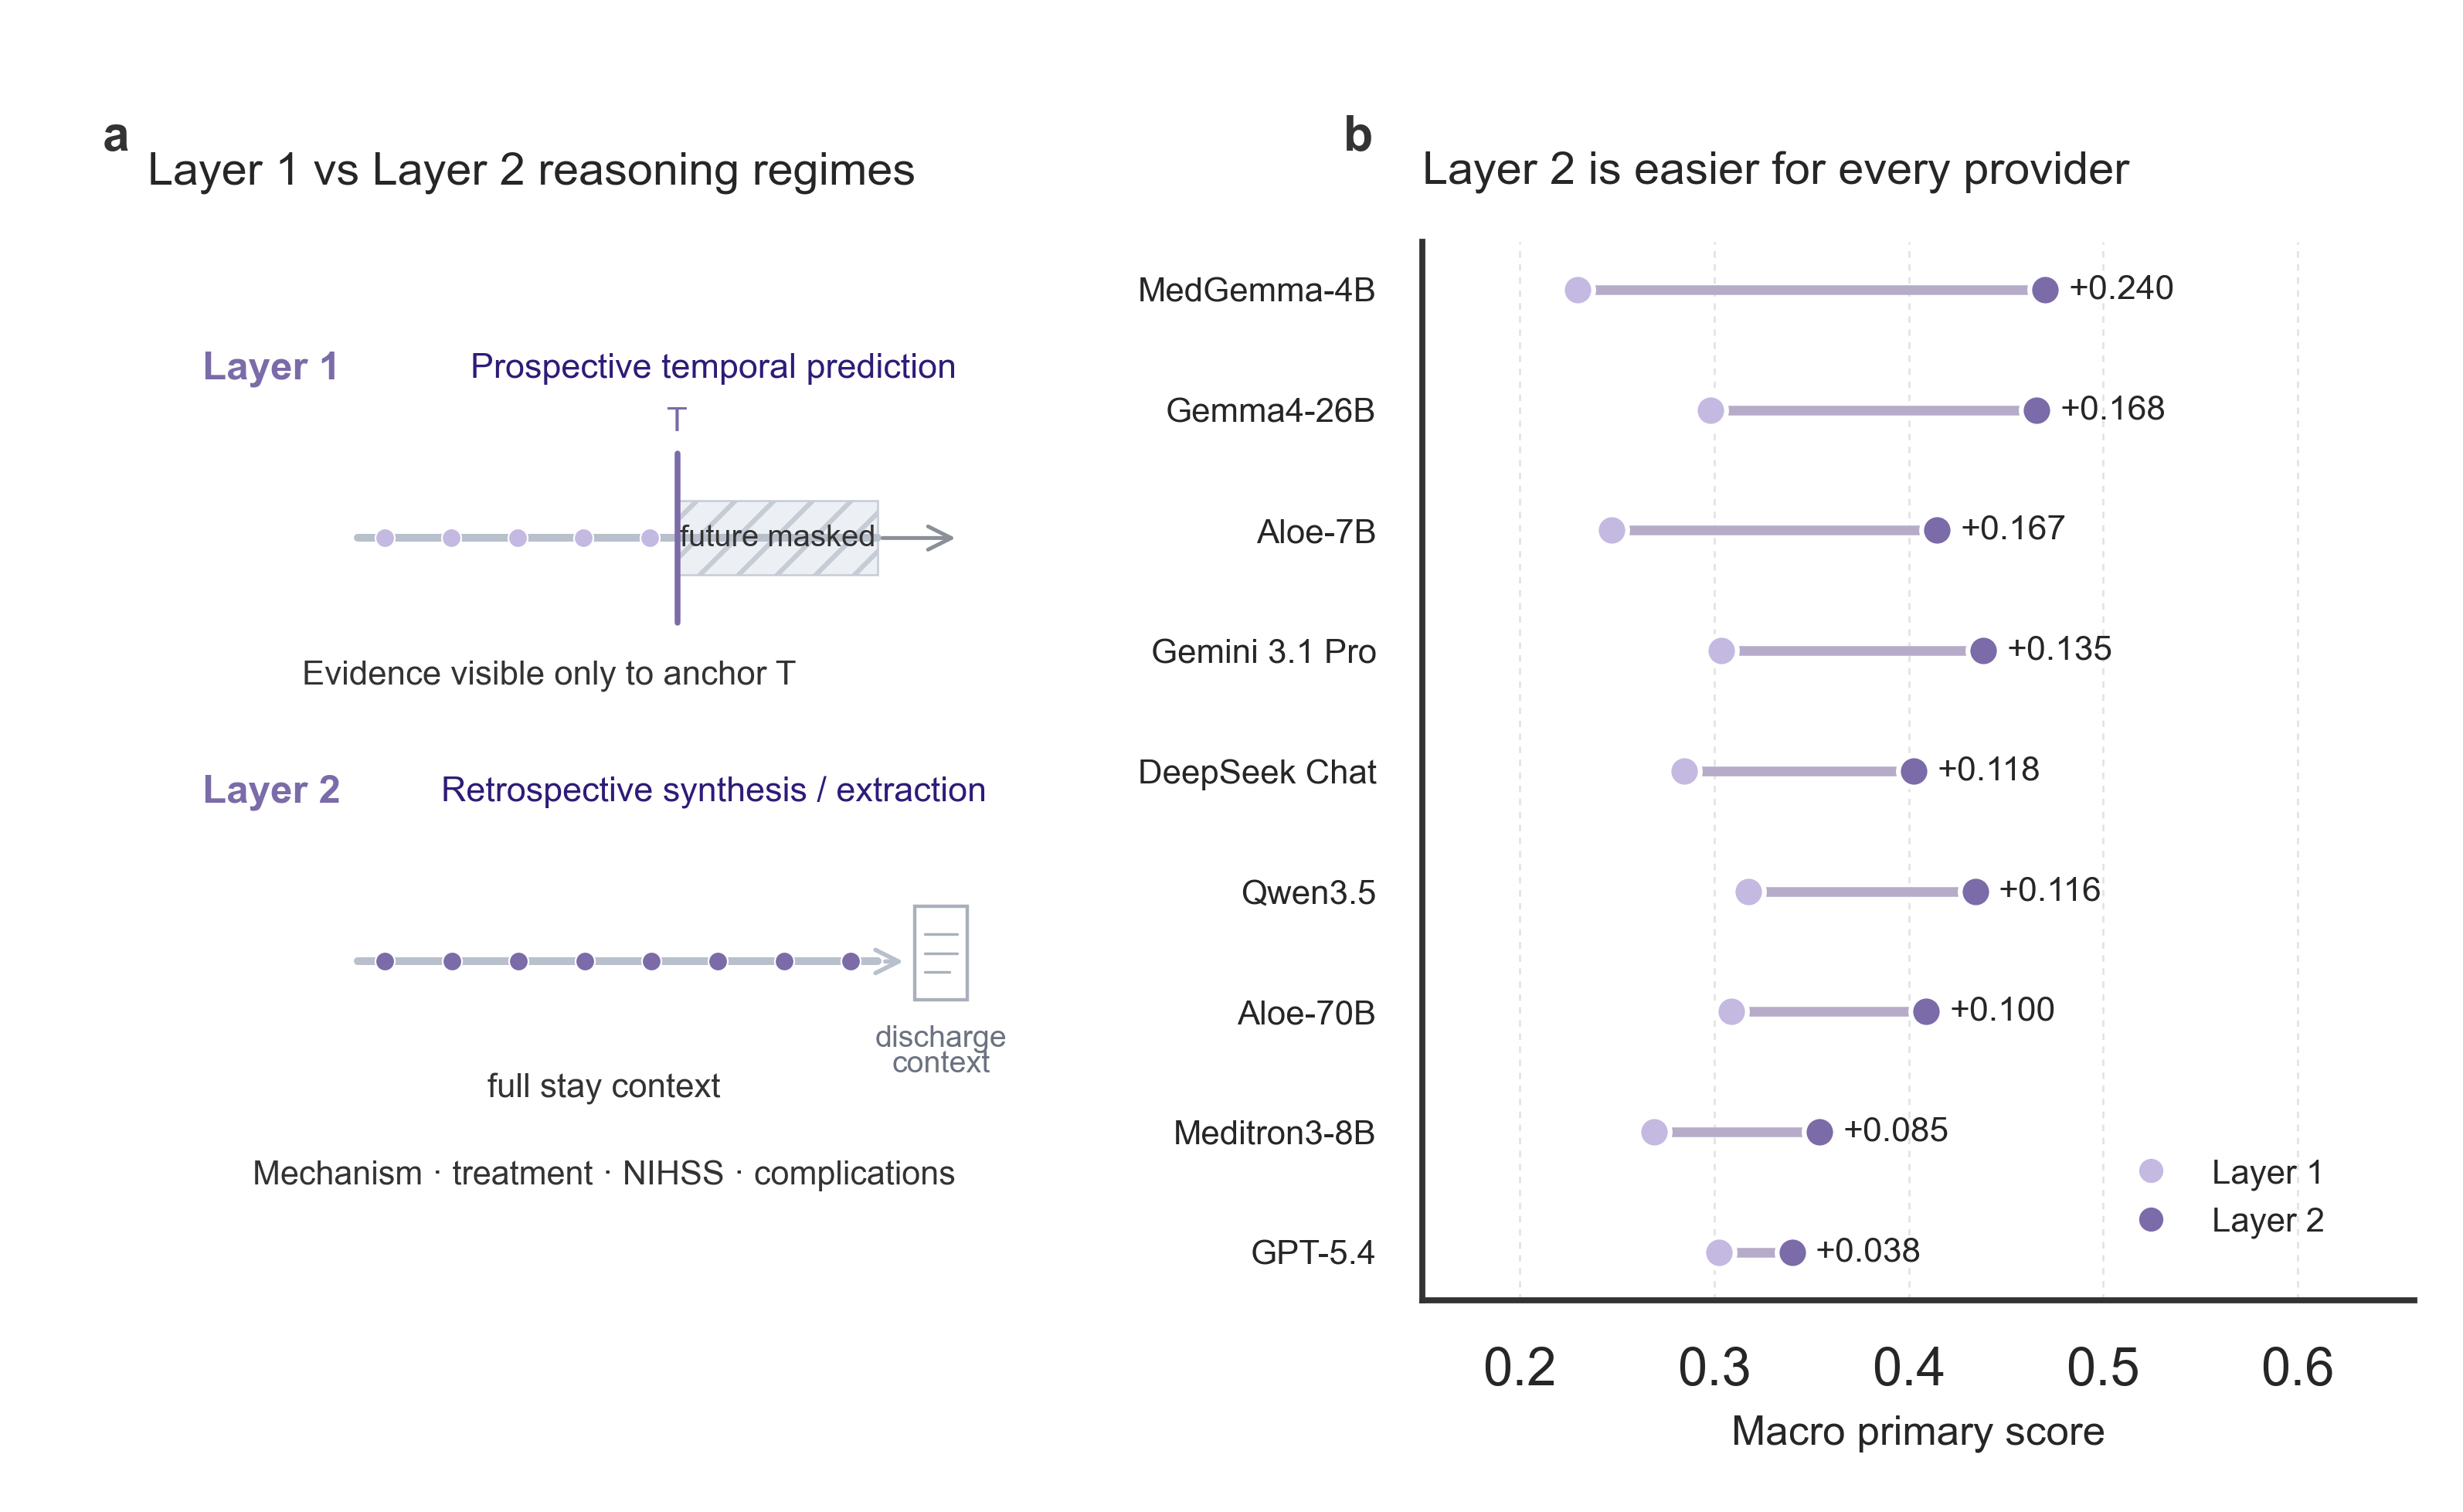
\includegraphics[width=\textwidth]{figures/main/figure5_stroke_layer_mechanism.png}
\caption{The stroke two-layer split captured a real reasoning boundary: retrospective synthesis and extraction were consistently easier than anchor-bounded temporal prediction. Panel a contrasts Layer 1, where only pre-anchor evidence is visible and the future neurological state is masked, with Layer 2, where full stay-level and discharge context support retrospective mechanism, treatment, NIHSS, and complication extraction. Panel b shows provider-level macro primary score for Layer 1 and Layer 2; Layer 2 outperformed Layer 1 for all nine providers. The mean Layer 2 minus Layer 1 gain was approximately +0.130 macro primary score.}
\label{fig:stroke_layers}
\end{figure*}

\FloatBarrier

\subsection{Template support revealed a strong trajectory gradient}

The trajectory-tier analysis tested whether physiology-template support identified clinically meaningful differences in trajectory difficulty.

Trajectory-tier analysis is one of the main methodological contributions of the benchmark because it links model performance to how well a stay matches an executable physiology template. Stay-level template-support coverage from the frozen Phase 5 summaries was 6\% for AKI, 96\% for delirium, and 37\% for sepsis (Fig.~\ref{fig:trajectory_tier}, panel a). These are not performance numbers; they quantify how often a stay could be matched with adequate support to the condition-specific template layer.

Row-level performance then varied systematically across trajectory tiers (Fig.~\ref{fig:trajectory_tier}, panel c). The gradient was strongest for delirium, intermediate for sepsis, and weakest for AKI. Template support is not a descriptive afterthought. It is a benchmark variable that tracks temporal interpretability. When the disease process aligns cleanly to an executable template, as in delirium, both phase labeling and downstream reasoning become easier. When template support is sparse, as in AKI, the resulting benchmark slice is more heterogeneous and harder to interpret.

AKI also produced one counterintuitive result: the low-support stratum outperformed the typical-supported stratum. This is not a scoring bug. The most plausible explanation is case-mix imbalance: low-support AKI cases contain more easy non-progression trajectories, whereas typical-supported AKI cases concentrate clinically dynamic stays that are harder to predict. The key point is not that typical support always implies higher performance, but that trajectory support exposes structure that would otherwise be invisible in pooled averages.

\begin{figure*}[t]
\centering
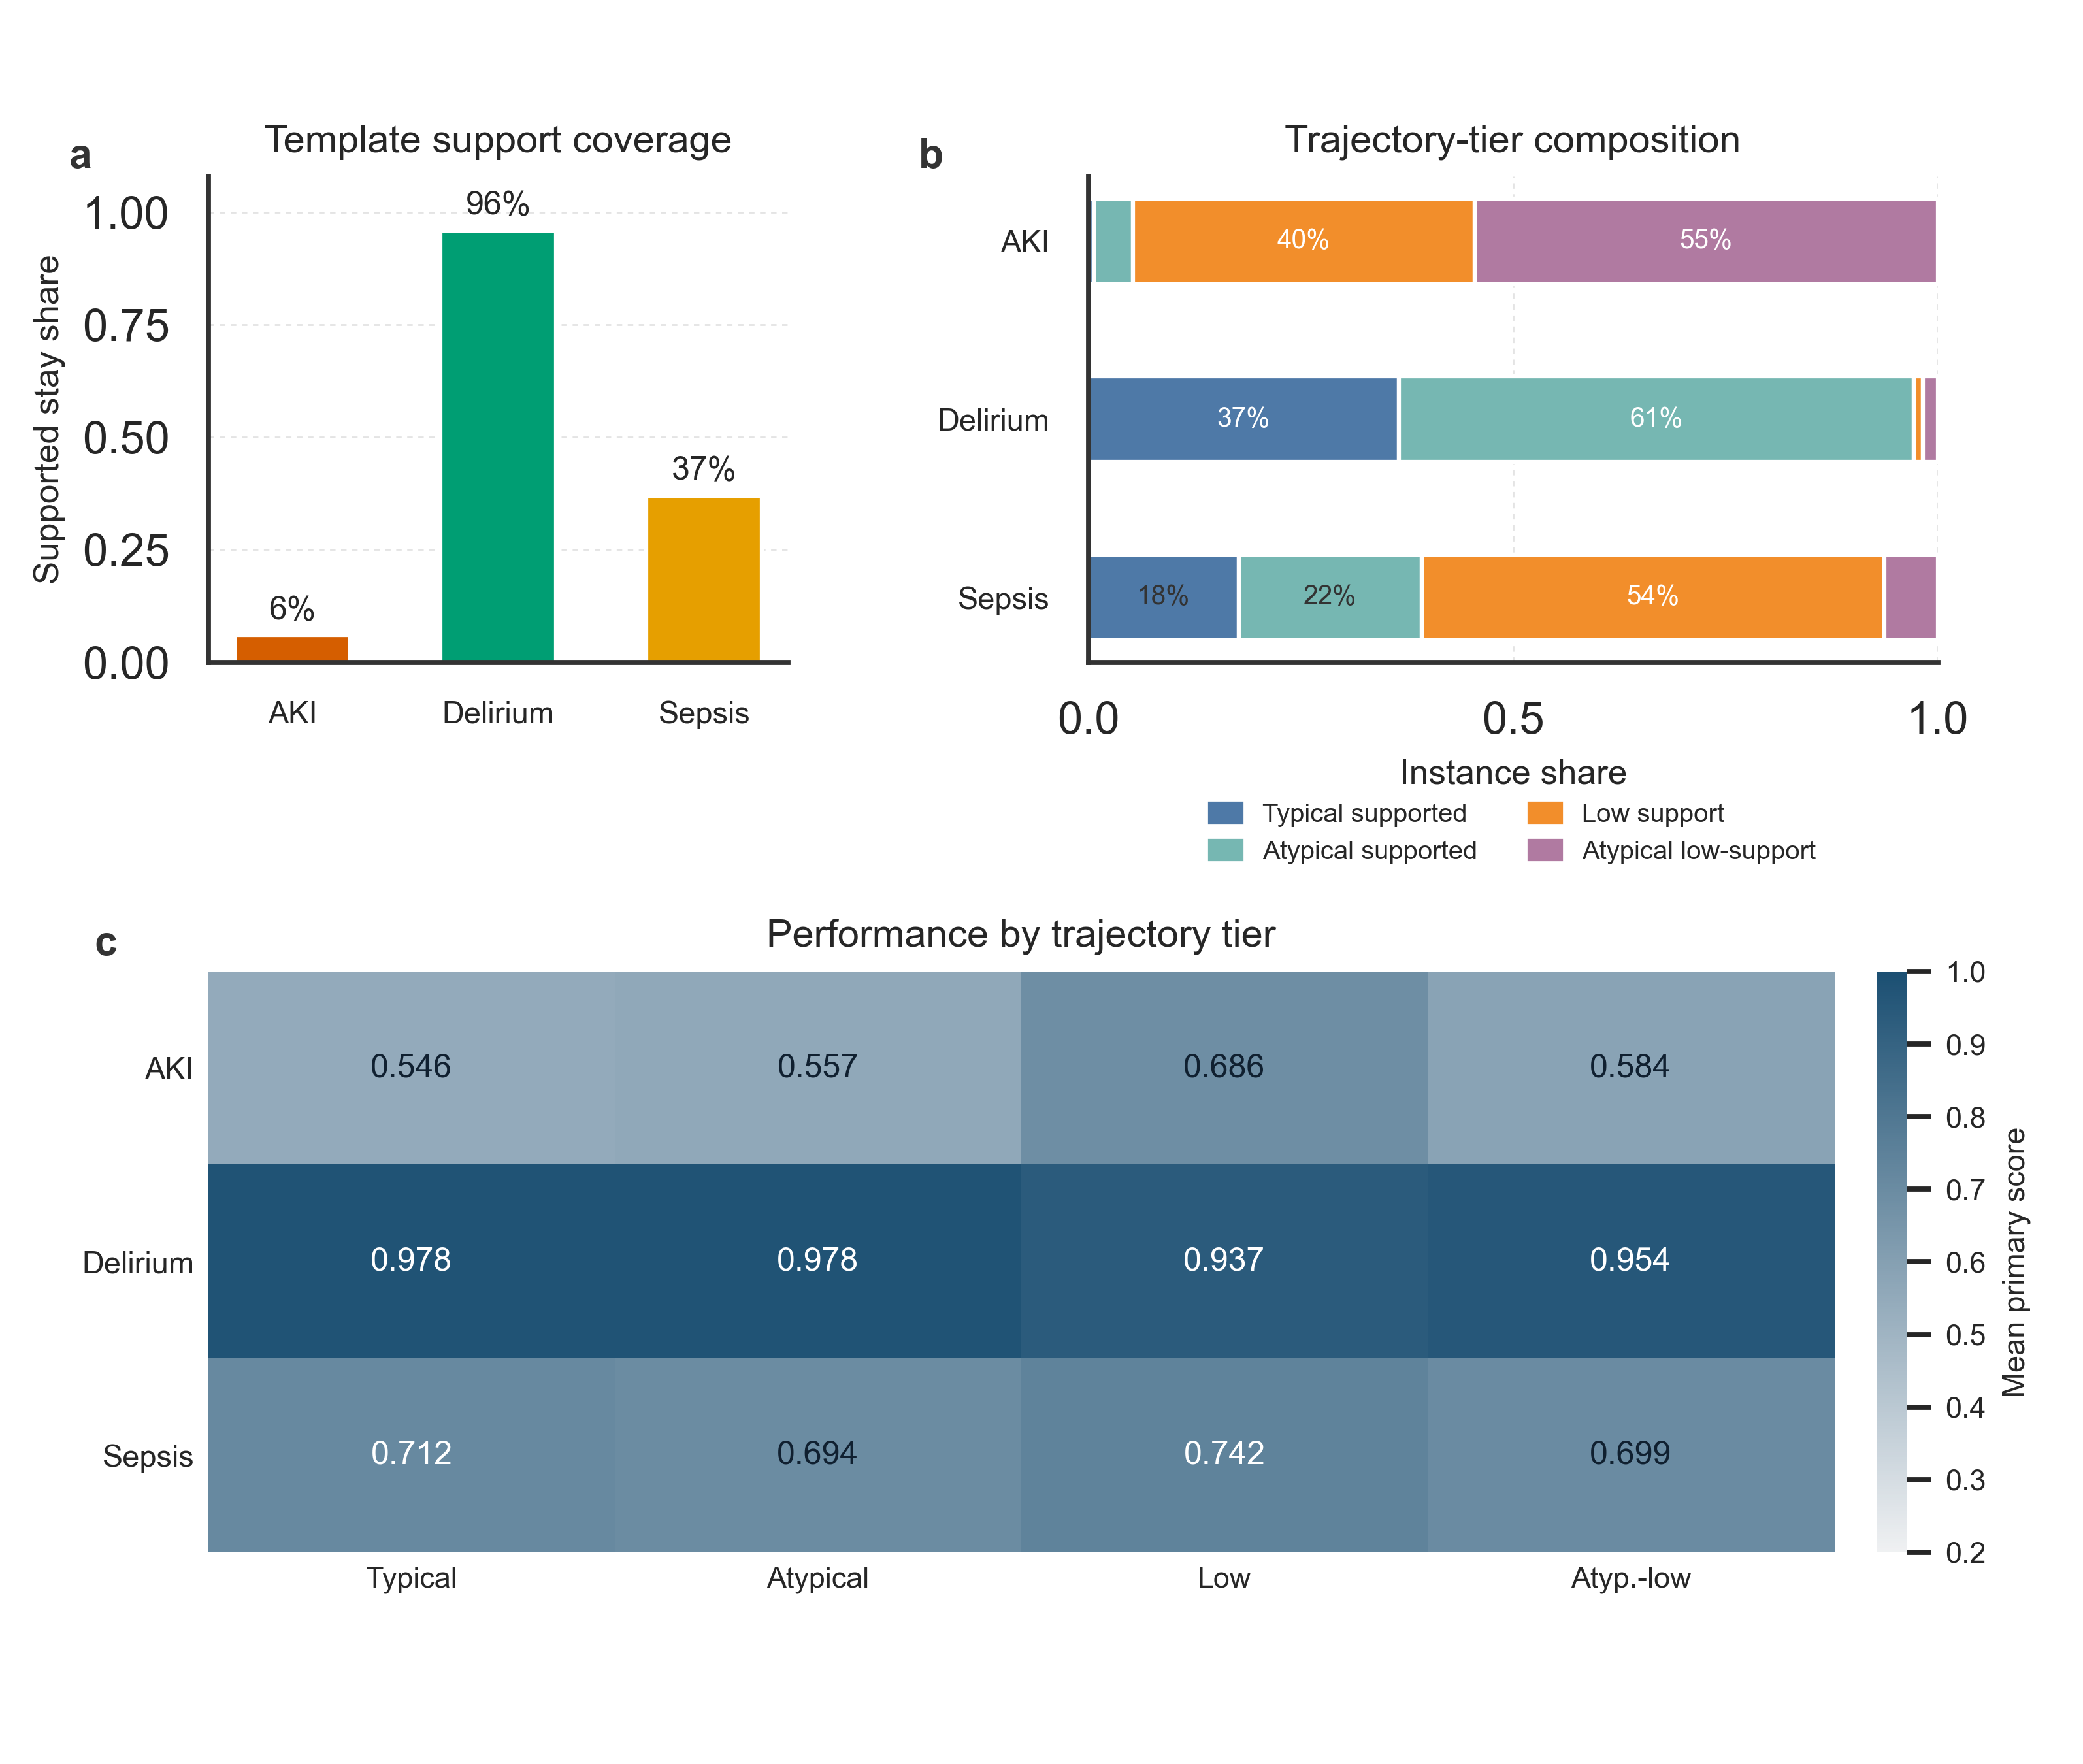
\includegraphics[width=\textwidth]{figures/main/figure6_template_state_space_stratification.png}
\caption{Template support revealed disease-specific trajectory regularity and exposed performance differences hidden in pooled averages. Panel a shows stay-level template support coverage for AKI, delirium, and sepsis. Panel b shows sample-instance composition across trajectory tiers; only major composition segments are labeled. Panel c shows row-level auto-scored mean primary score by trajectory tier. Template support is an evidence-support / templatability measure, not a model-performance metric. The higher score in the AKI low-support stratum likely reflects easier non-progression case mix rather than a universal benefit of low support.}
\label{fig:trajectory_tier}
\end{figure*}

\FloatBarrier

\subsection{Judge-based evaluation preserved the auto-scored provider ordering}

The judge phase checked whether the auto-scored ordering persisted when open-ended response quality was assessed on deferred and hard-disagreement cases.

Judge evaluation was intentionally restricted to a fixed four-model contestant roster: GPT-5.4, DeepSeek Chat, Aloe-70B, and MedGemma-4B. The packet contained 500 prompt instances and 2,000 contestant responses, scored primarily by Claude Opus 4.6 with GPT-5.4 and Gemini 3.1 Pro as cross-check judges. The purpose was not to replace auto-scoring, but to evaluate higher-level response quality on a controlled subset that mixed deferred items and hard auto-scorable disagreements.

Judge summaries preserved the same broad provider separation seen in auto-scoring (Table~\ref{tab:judge_provider_summary}; Fig.~\ref{fig:judge_provider_summary}). Reported summary values average the scores assigned by Claude Opus 4.6, GPT-5.4, and Gemini 3.1 Pro on the same response rows. GPT-5.4 led on all five rubric axes, followed by DeepSeek Chat, then Aloe-70B, with MedGemma-4B last. The ordering did not depend on one parser or one metric family. It remained visible when the evaluation target shifted from auto-scored correctness to graded quality, clinical correctness, temporal grounding, evidence grounding, and confidence calibration.

Cross-judge agreement was substantial (Table~\ref{tab:judge_agreement}). Against the primary judge, GPT-5.4 achieved Spearman $\rho$ 0.814 on overall quality and 0.808 on clinical correctness. Gemini's corresponding cross-check values were 0.783 and 0.759. These values support the judge phase as a structured complementary evaluation layer, while still requiring explicit disclosure that GPT-5.4 appeared both as a contestant and as one cross-check judge.

\begin{figure*}[t]
\centering
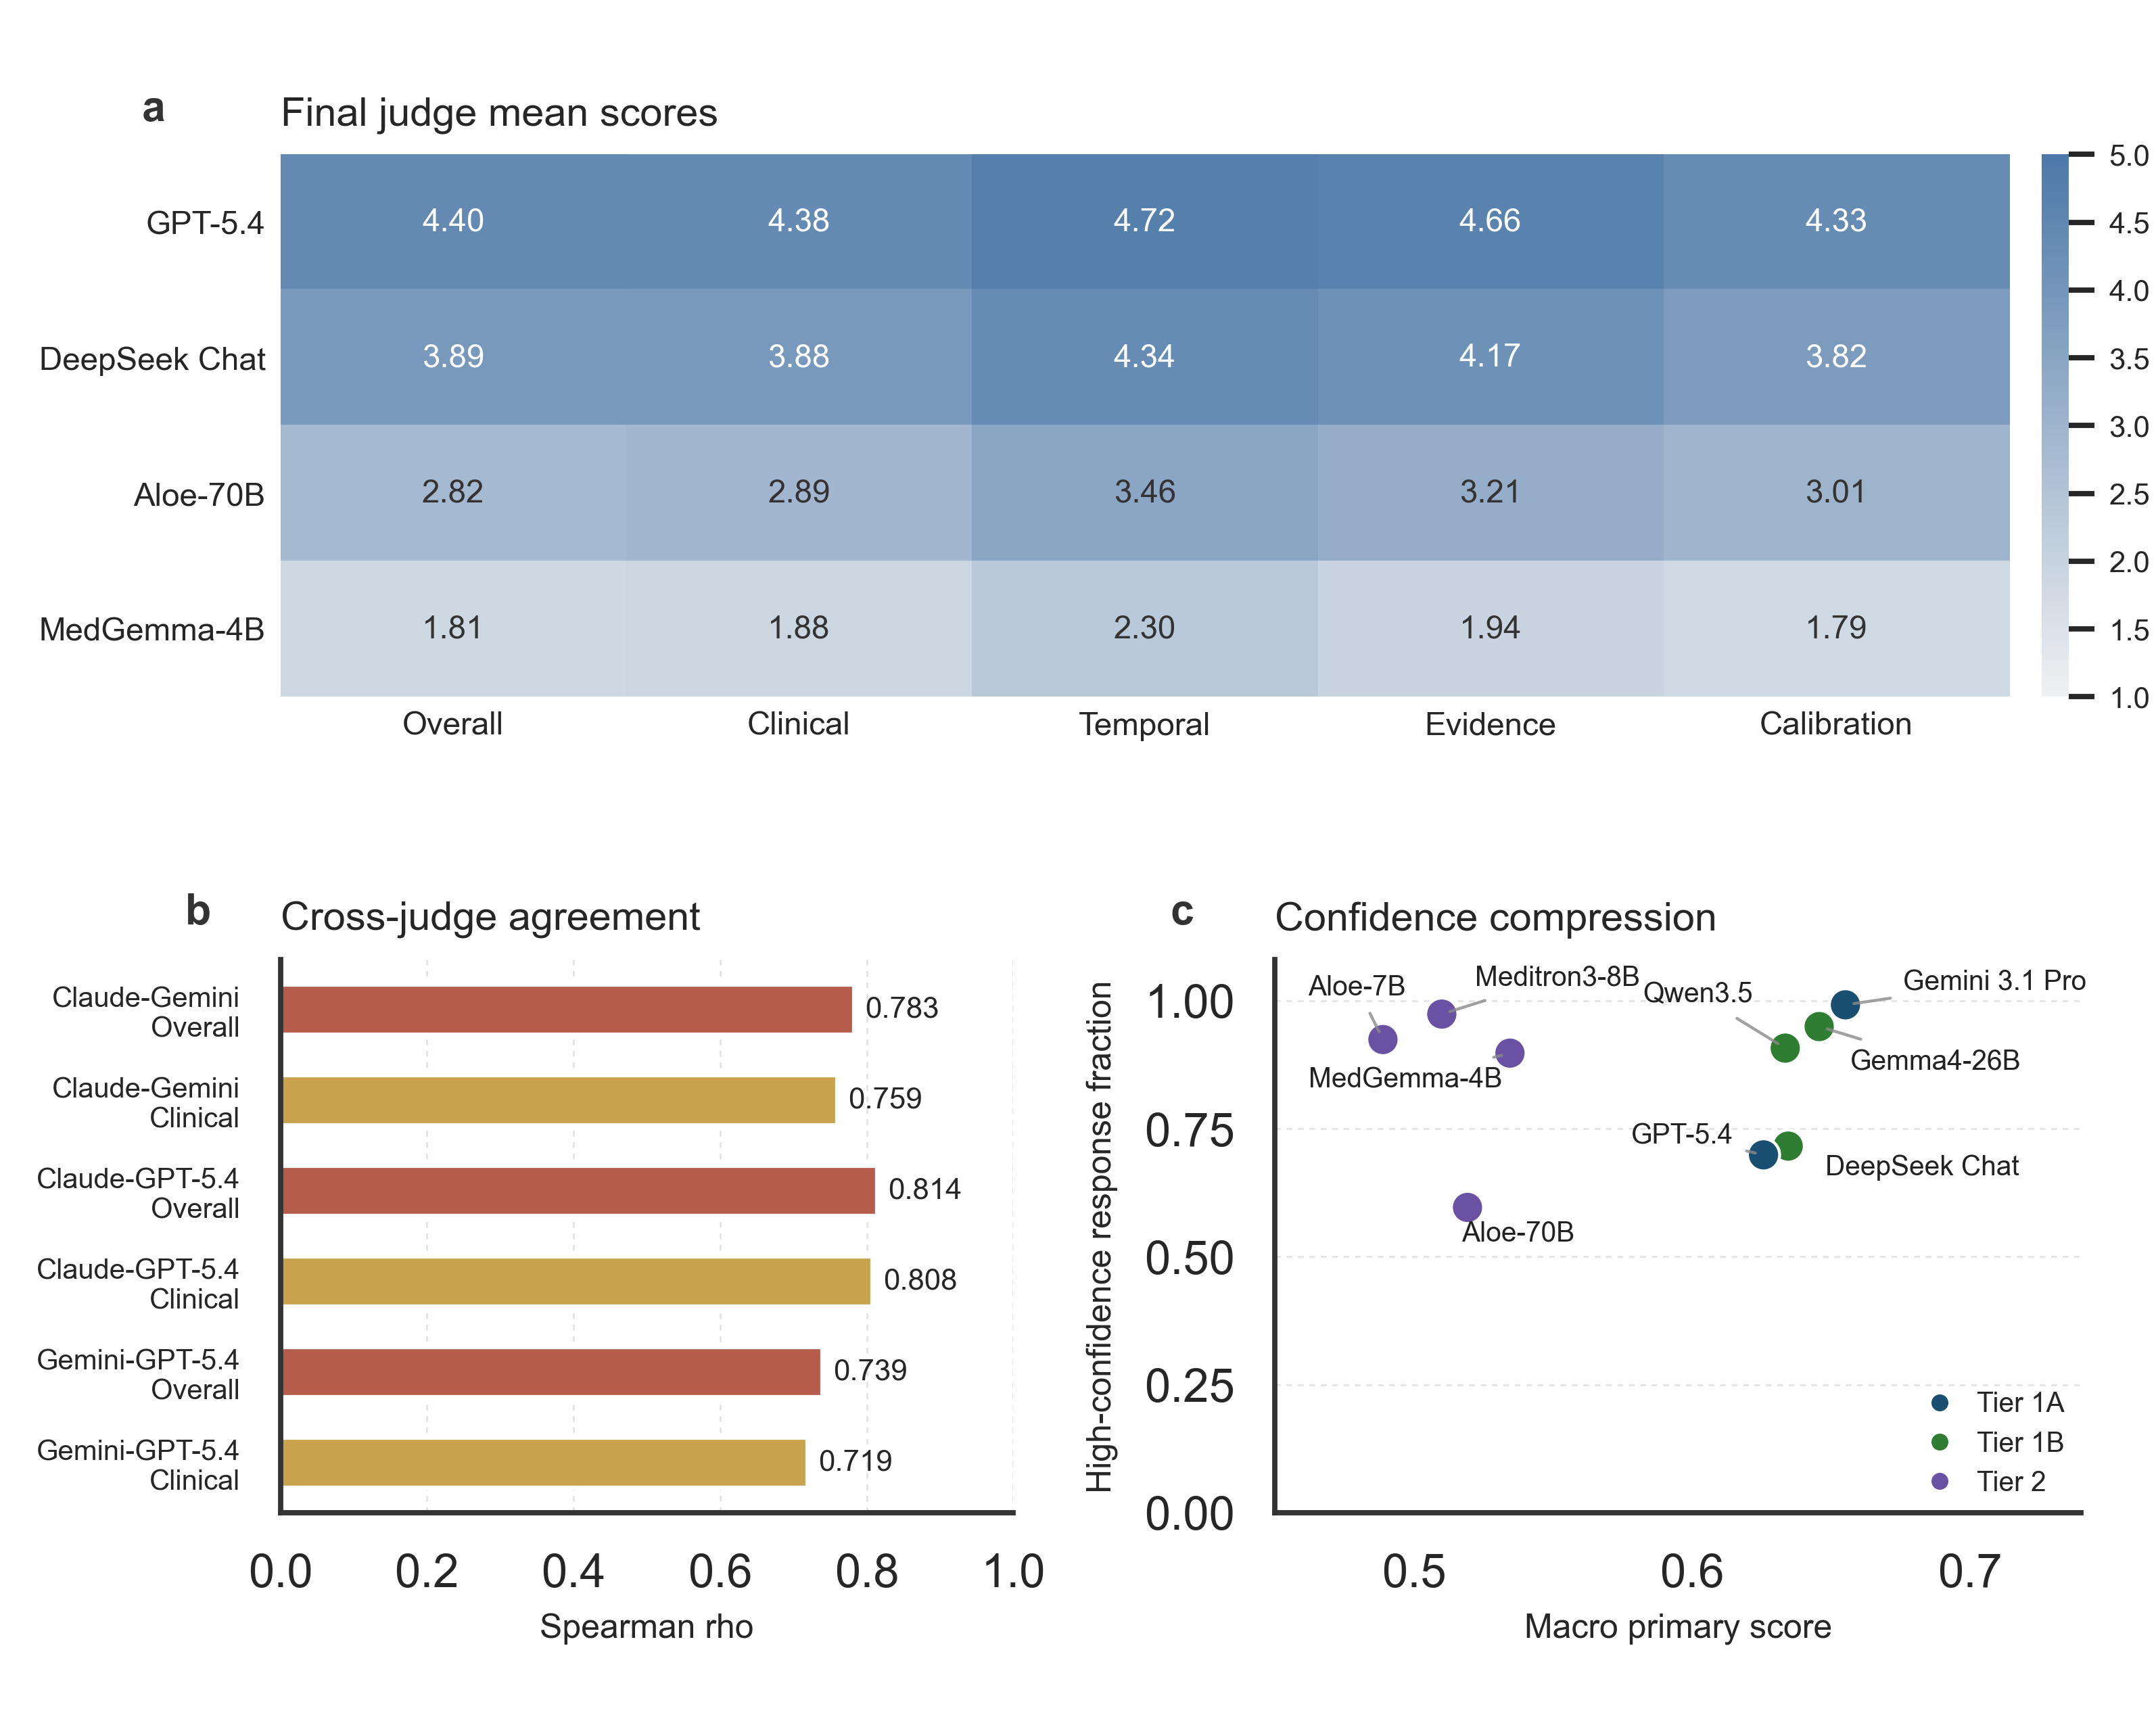
\includegraphics[width=\textwidth]{figures/main/figure7_judge_validation_calibration.png}
\caption{Judge-based evaluation preserved the broad provider ordering while revealing differences in response quality and confidence behavior. Panel a reports final mean scores across the three judges for overall quality, clinical correctness, temporal grounding, evidence grounding, and calibration for the four fixed judge-phase contestants. Panel b shows pairwise cross-judge Spearman correlations for overall quality and clinical correctness. Panel c compares overall macro primary score with the fraction of high-confidence responses across all nine providers; all provider points are labeled. Confidence fraction uses full 53,070-prompt provider summaries where available and is the share of parsed responses with \texttt{confidence\_value} equal to high, not statistical probability calibration. The judge packet contained 500 prompt instances and 2,000 contestant responses, evaluated by Claude Opus 4.6, GPT-5.4, and Gemini 3.1 Pro on the same rows.}
\label{fig:judge_provider_summary}
\end{figure*}

\begin{table*}[t]
\caption{Judge-based provider summary for the four fixed contestants, reporting mean rubric scores across the three judges on a 1--5 scale.}
\label{tab:judge_provider_summary}
\centering
\scriptsize
\begin{tabular}{@{}lrrrrr@{}}
\toprule
Provider & Overall & Clinical & Temporal & Evidence & Calibration \\
\midrule
GPT-5.4 & 4.397 & 4.383 & 4.722 & 4.655 & 4.325 \\
DeepSeek Chat & 3.894 & 3.882 & 4.342 & 4.167 & 3.819 \\
Aloe-70B & 2.823 & 2.885 & 3.464 & 3.209 & 3.008 \\
MedGemma-4B & 1.813 & 1.883 & 2.298 & 1.945 & 1.793 \\
\botrule
\end{tabular}
\normalsize
\end{table*}


\begin{table*}[t]
\caption{Judge agreement summary across the shared 2,000-row judge packet.}
\label{tab:judge_agreement}
\centering
\scriptsize
\begin{tabular}{@{}lllrrr@{}}
\toprule
Judge A & Judge B & Score & Rows & Spearman $\rho$ & Exact match rate \\
\midrule
Claude Opus 4.6 & Gemini 3.1 Pro & overall quality & 2000 & 0.783 & 0.283 \\
Claude Opus 4.6 & Gemini 3.1 Pro & clinical correctness & 2000 & 0.759 & 0.286 \\
Claude Opus 4.6 & GPT-5.4 & overall quality & 2000 & 0.814 & 0.527 \\
Claude Opus 4.6 & GPT-5.4 & clinical correctness & 2000 & 0.808 & 0.511 \\
Gemini 3.1 Pro & GPT-5.4 & overall quality & 2000 & 0.739 & 0.410 \\
Gemini 3.1 Pro & GPT-5.4 & clinical correctness & 2000 & 0.719 & 0.411 \\
\botrule
\end{tabular}
\normalsize
\end{table*}


\FloatBarrier

\section{Discussion}

Four findings stand out. Temporal clinical reasoning difficulty was strongly condition-dependent (RQ2): delirium was near ceiling for several providers, whereas stroke remained difficult for all tiers. Explicit temporal sequence modeling did not uniformly outperform a compact structured summary representation (RQ1). General-purpose models led the aggregate ranking, while medical-domain models remained below the Tier 1A and Tier 1B groups overall (RQ3). Trajectory-template support also carried information about reasoning difficulty and should be reported in temporal clinical benchmarks (RQ2).

The branch comparison matters because temporal richness is often assumed to be beneficial. Our results do not support that generalization. Branch B1 improved AUROC on only 3 of 7 eligible tasks and AUPRC on only 1 of 7. The most defensible interpretation is that temporal structure helps only when it aligns with the task's decision boundary and is represented in a recoverable way. For some tasks, a strong anchor-state summary was sufficient, or even preferable.

The aggregate tier gap between general-purpose and medical-domain models is the most consequential benchmark-level finding. At the aggregate benchmark level, all four Tier 2 models underperformed the Tier 1A and Tier 1B groups, although condition-level rankings still showed local variation. This directly addresses whether medical-domain fine-tuning improves longitudinal multimodal reasoning. On TIMELY Bench, it did not at the aggregate benchmark level. Current medical adaptation appears better aligned to medical question answering and knowledge recall than to anchor-bounded temporal interpretation of evolving evidence. This pattern is consistent with broader clinical LLM evaluations showing that strong medical knowledge encoding does not automatically translate into robust open-ended clinical decision making\cite{singhal2023clinicalknowledge,hager2024clinicaldecision}. It also supports the argument that generalist medical AI will require flexible multimodal reasoning and clinically relevant validation, not simply domain-specific vocabulary or benchmark-tuned medical QA performance\cite{moor2023gmai,saab2024gemini}.

This finding is most informative when placed beside existing medical benchmarks. MedQA and PubMedQA remain important tests of medical knowledge use and biomedical text reasoning, but their prompts do not require synchronized interpretation of structured measurements, medications, procedures, and notes across a masked timeline\cite{jin2021medqa,jin2019pubmedqa}. HealthBench, MedHELM, and LLMEval-Med represent a newer generation of clinically grounded LLM evaluations that use open-ended responses, physician-informed rubrics, broad task taxonomies, or real-world clinical cases\cite{arora2025healthbench,bedi2025medhelm,zhang2025llmevalmed}. Their contribution is breadth and clinical realism across conversations, tasks, or cases. TIMELY Bench is narrower, but it goes deeper on one axis: anchor-bounded temporal reasoning from synchronized ICU trajectories. EHRSHOT emphasizes few-shot transfer on coded longitudinal records, not multimodal trajectory reasoning\cite{wornow2023ehrshot}. MedAgentBench reports a best-model task success rate of 69.67\% for interactive medical agents, which is useful for understanding tool use and workflow execution, but it answers a different question from TIMELY Bench\cite{jiang2025medagentbench}. MedAgentBench asks whether an agent can act within a virtual EHR environment. TIMELY Bench asks whether a model can correctly interpret a bounded patient trajectory under matched information states. These benchmark families are complementary, not interchangeable.

The comparison also helps explain why Tier 2 underperformance should not be dismissed as a benchmark quirk. Medical-domain models such as Me-LLaMA and MEDITRON were designed to strengthen clinical language competence and downstream medical task performance\cite{xie2025mellama,chen2023meditron}. Benchmarks such as MedQA, PubMedQA, and agentic EHR tasks reward capabilities that domain tuning plausibly improves: clinical vocabulary, factual retrieval, treatment-pattern familiarity, and medical discourse modeling. TIMELY Bench stresses a different composite skill: bounded longitudinal interpretation under synchronized multimodal evidence. Our results suggest that present-day medical fine-tuning is useful for fluent clinical language use but insufficient for robust temporal clinical reasoning.

The per-dimension results sharpen that comparison. D3 trend reasoning was comparatively strong, D2 threshold reasoning separated tiers sharply, and D4 diagnostic discrimination was weak across the board. Current models can often detect directional change once the signal is explicit, but still struggle when the task requires choosing among alternative clinical explanations. The weakest dimension was diagnostic interpretation under partially overlapping evidence, not raw time indexing. That is closer to real clinical reasoning than a generic accuracy leaderboard can show.

Self-reported confidence behavior adds another layer to this picture. Gemini 3.1 Pro achieved the highest overall macro primary score, yet marked 99.2\% of prompts as high confidence. GPT-5.4, by contrast, used the high-confidence label in 69.9\% of prompts. This divergence matters for deployment-oriented digital medicine because a model that is correct but nearly always maximally confident may be harder to supervise in uncertainty-aware workflows. Future medical LLM evaluations should report confidence behavior alongside correctness, particularly for models intended for clinical triage or decision support.

The clinical significance of TIMELY Bench is not that it identifies a single deployable model. It provides a way to ask clinically sharper questions before deployment: whether a model can reason only from evidence available at an ICU decision time, whether it can distinguish a threshold crossing from a nonspecific abnormality, whether it recognizes atypical or low-support trajectories, and whether it can abstain when the visible evidence is insufficient. These properties are close to the requirements of real clinical decision support, where incorrect early warning, overconfident escalation, or retrospective leakage can each create different harms. The AKI and sepsis task designs connect directly to prior work on continuous AKI prediction and prospective sepsis alerting, but shift the emphasis from risk score performance to interpretable reasoning under an explicit information state\cite{tomasev2019aki,adams2022trews}.

Although TIMELY Bench is not an operational tool for trial recruitment, safety review, or rare disease discovery, the same evaluation logic is relevant to translational uses of longitudinal EHR data. Drug development increasingly uses real-world data to identify trial-eligible patients, characterize disease progression, and support endpoint or safety-event abstraction, but these tasks depend on whether an event was identifiable from evidence available at the relevant time rather than from retrospective knowledge\cite{fda2023rwe,richesson2013ehrphenotyping}. TIMELY Bench does not validate models for clinical trial operations or regulatory use. It provides a pre-deployment evaluation scaffold for testing whether a model respects the information boundary at an anchor, localizes event onset, detects threshold crossing, and attributes its answer to visible evidence. Similar requirements arise in pharmacovigilance, where adverse events such as AKI, sepsis, delirium, and drug-related organ injury emerge through evolving laboratory values, treatments, vital signs, and clinical notes rather than through a single isolated observation\cite{wang2009pharmacovigilance,harpaz2012adverseevent}. The CRES dimensions map naturally onto these safety-review questions: when did the event become visible, which threshold or trend changed, and which observations support the judgment? Finally, the physiology-template layer suggests a future extension for rare disease research, where natural history studies and phenotype discovery often require longitudinal interpretation of sparse, heterogeneous records\cite{fda2019rarediseasehistory,bastarache2018phers}. Disease-specific templates could define phases, trajectory tiers, and atypical variants, then evaluate whether models can recognize progression patterns from partial EHR evidence.

Trajectory-template support is also a methodological contribution in its own right. Delirium, sepsis, and AKI did not simply differ in overall performance. They differed in how often their stays could be cleanly mapped onto executable physiology templates and in how strongly that support gradient separated model behavior. The extreme difference between delirium (96\% stay-level support) and AKI (6\%) indicates that disease-specific temporal regularity is part of the benchmark construct, not merely an implementation detail. Future temporal clinical benchmarks should report task distributions and how much of the trajectory space is clinically templatable.

This study has several limitations. TIMELY Bench is retrospective and derived from a single source environment, so it does not establish transportability across institutions, documentation cultures, or EHR systems. Stroke currently bypasses the B3 template layer, which means the four condition families are not perfectly symmetric at the latent-state level.

Judge evaluation remains model-based rather than human-adjudicated; although LLM-as-judge methods are increasingly used for open-ended medical evaluation, they remain a complement to, not a substitute for, expert human adjudication\cite{zheng2023judging,bedi2025medhelm}. Cross-condition causal pathways such as septic AKI and septic encephalopathy are not modeled in the current template layer. Each condition family is evaluated as an independent track, and multimorbidity reasoning across conditions represents a natural extension for future benchmark versions. The delirium anchor relies on CAM-ICU assessments (item 228332), which may systematically underrepresent hypoactive delirium subtypes that are clinically present but not captured by the screening tool. The benchmark mitigates this through explicit left-censoring flags and stratified reporting, but the underlying ascertainment bias is inherent to the instrument rather than fully correctable at the benchmark level. SOFA decomposition in the sepsis condition currently covers four of six organ components (respiratory, cardiovascular, renal, and hepatic); neurological and coagulation components are not yet fully materialized in the current state vectors and should be added in future iterations.

The benchmark does not include prospective evaluation in live clinical workflows. Any future interventional use would require prospective protocol and trial reporting aligned with AI-specific guidance such as SPIRIT-AI and CONSORT-AI\cite{rivera2020spiritai,liu2020consortai}.

Taken together, these results support TIMELY Bench as a diagnostic instrument for temporal clinical AI evaluation. It frames temporal reasoning as a condition-aware, anchor-bounded, multi-representation problem, exposes when temporal structure helps and when it does not, and makes disease-specific trajectory support visible. That role is narrower than clinical deployment, but broader than a leaderboard.

\section{Methods}

\subsection{Study design and source data}

TIMELY Bench was constructed as a phase-locked benchmark for temporal clinical reasoning over ICU data derived from MIMIC-IV v3.1 and MIMIC-IV Note\cite{johnson2023mimic}. Source tables were accessed through the credentialed PhysioNet BigQuery distribution, including ICU, hospital, derived, discharge-note, and radiology-note modules. The full pipeline comprised six stages: (1) hourly alignment of structured and textual evidence onto a shared 168-hour grid; (2) construction of executable physiology templates for AKI, delirium, and sepsis; (3) materialization of synchronized representation branches; (4) condition-specific Clinical Reasoning Evaluation Suite (CRES) assembly; (5) state-space reconstruction with phase labeling and trajectory-tier assignment; and (6) frozen benchmark release, evaluation, canonicalization, and comparative scoring. The present study is retrospective and methodologically aligned to STROBE, RECORD, and MI-CLAIM reporting domains\cite{vonelm2007strobe,benchimol2015record,norgeot2020miclaim}.

The benchmark was anchor-bounded by design. Every prompt instance corresponds to one stay, one task, one reasoning dimension, and one anchor hour. All evidence visible to the model is truncated to the interval from ICU admission through that anchor, and all future information is masked. This prevents the benchmark from conflating temporal reasoning with inadvertent future leakage and allows the same stay to be evaluated under multiple information states.

This study used de-identified data from MIMIC-IV v3.1 and MIMIC-IV Note, available through the PhysioNet credentialed data access program and its BigQuery-hosted release. Access requires completion of a recognized human subjects training course and signing of a data use agreement. The MIMIC-IV dataset was collected under a waiver of informed consent approved by the Beth Israel Deaconess Medical Center institutional review board. No additional ethical approval was required for this secondary analysis of de-identified data. This study did not involve any prospective data collection, patient contact, or intervention.

\subsection{Hourly alignment and synchronized representations}

Phase 1 aligned heterogeneous EHR sources to an hourly grid spanning the first 168 ICU hours. Structured observations, medications, procedures, diagnosis-pathway events, and note fragments were each mapped to hourly or event-time representations. The benchmark then materialized four synchronized views of the same stay and anchor.

Branch A is a compact structured summary intended for conventional machine-learning baselines. Branch B1 preserves an explicit hourly sequence of structured observations suitable for recurrent or transformer models. Branch B2 is the prompt-ready multimodal EHR representation used for LLM evaluation; in this paper, multimodal denotes EHR modalities rather than imaging or audio, including structured measurements, medications, procedures, clinical notes, and condition-specific observations. The underlying time-aware context object stores a broader set of structured hourly features, while final prompt serialization renders a condition-specific subset according to the evaluation policy. Branch B3 reconstructs a low-dimensional state-space over time and serves as the input to Phase 5 template application for AKI, delirium, and sepsis. Because the four branches are synchronized to the same stay and anchor, they allow direct representation-level comparisons without changing the underlying patient state.

Phase 5 did not attempt to infer a fully latent disease mechanism from free text. Instead, it applied condition-specific executable rules derived from the Phase 2 physiology templates to B3 trajectories. These rules converted hourly state vectors into coarse phase labels and trajectory tiers using the template-defined phase windows, expected marker trajectories, and atypical variants. Template support scores in the frozen release quantify observation coverage within phase-aligned time windows rather than full semantic trajectory matching. A high support score therefore means that the required marker observations were sufficiently present for a template-aligned rule to be applied; it does not mean that the full clinical narrative was proven to follow an idealized trajectory. This distinction is central to interpreting the trajectory-tier analysis.

\subsection{Condition definitions and label construction}

\noindent\textbf{AKI.} AKI cohort construction relied on the derived \texttt{kdigo\_stages} table and restricted the source cohort to stays with AKI evidence. Physiology templates anchored AKI onset to the first hour meeting KDIGO Stage 1 criteria: serum creatinine increase of at least 0.3 mg/dL within 48 hours, serum creatinine at least 1.5 times baseline, or urine output below 0.5 mL/kg/h for at least 6 hours\cite{kdigo2012aki}. This choice follows the same clinical motivation as continuous AKI early-warning systems, where the relevant question is whether deterioration can be recognized with enough lead time to act rather than whether an already completed episode can be summarized retrospectively\cite{tomasev2019aki}. Only stays with Stage 1 onset within the first 48 ICU hours were retained for the main AKI task build. Phase 3 extracted Stage 1, Stage 2+, and Stage 3 onset hours from the derived table, then added renal replacement therapy (RRT) proxy timing from procedure events and hourly-grid RRT indicators. Temporal anchors were emitted every 4 hours starting at \texttt{stage1\_onset\_hour + 4}. For AKI-T1, the row label is positive if Stage 2+ onset falls in $(T, T+24]$; for AKI-S1, the row label is positive if an RRT proxy event falls in $(T, T+72]$. Anchors after the first observed progression or RRT proxy event are not retained, which ensures that each prompt corresponds to a genuinely pre-escalation information state rather than a retrospective restatement of already visible failure.

\noindent\textbf{Delirium.} Delirium onset was anchored to the first positive CAM-ICU assessment, operationalized from MIMIC charted delirium assessments (itemid 228332) with the requirement that the patient be assessable at RASS $\geq -3$\cite{ely2001camicu}. The template construction was intended to approximate DSM-5 delirium constructs while remaining executable on hourly ICU observations rather than on bedside neuropsychiatric examination narratives\cite{apa2013dsm5}. The Phase 2 delirium template defined the anchor event as a first CAM-ICU positive state requiring Feature 1 and 2 plus either 3 or 4. Phase 3 combined the delirium cohort, delirium labels, neurological hourly features, GCS features, and restraint features to derive both metadata and task labels. Each task row inherits the hourly delirium-label grid and carries a fixed 24-hour look-ahead horizon. DEL-T1 captures persistent delirium within $(T, T+24]$, whereas DEL-S1 captures resolution within $(T, T+24]$ using a sustained 24-hour non-positive window. In addition to the binary label, the task table carries \texttt{left\_censored}, counts of positive and negative delirium hours, and support flags for RASS, GCS, and restraints so that evaluation can separate physiology from observation sparsity. Left-censoring was retained as an explicit field because some stays entered observation after part of the trajectory had already unfolded.

\noindent\textbf{Sepsis.} Sepsis cohort construction started from stays flagged \texttt{sepsis3} in the source cohort and then derived onset timing from diagnosis-pathway events. If the pathway stream contained an event whose name included both \texttt{sepsis} and \texttt{onset}, the earliest such hour became the sepsis onset. If no explicit onset event was found, the onset hour was set to zero and the stay was marked with \texttt{onset\_confidence=low}; otherwise onset confidence was \texttt{high}. Septic shock was operationalized from hourly features as mean arterial pressure below 65 mmHg with active vasopressor support, with lactate $>2$ mmol/L used as an additional gate when lactate was available, consistent with Sepsis-3 shock criteria and Surviving Sepsis Campaign guidance\cite{singer2016sepsis3,evans2021surviving}. The task design intentionally mirrors the clinical deployment problem studied in sepsis early-warning systems such as TREWS: recognizing high-risk evolution before treatment opportunities have passed, while retaining enough provenance to audit which evidence was available at alert time\cite{adams2022trews}. Prediction anchors were emitted every 4 hours starting at \texttt{sepsis\_onset\_hour + 4}. For SEP-T1, labels are positive when the first post-onset septic-shock hour lies in $(T, T+12]$; anchors at or after an already observed shock hour are excluded. For SEP-S1, the baseline lactate at hour $T$ must be observed and positive, and the label is positive if the minimum future lactate in $(T, T+6]$ drops to at most 90\% of baseline. The metadata table also records whether shock occurred before or exactly at sepsis onset and whether the stay had lactate, vasopressor, and SOFA support, which is important because many sepsis failures are support-availability failures rather than pure reasoning failures.

\noindent\textbf{Stroke.} Stroke construction used a stricter phenotype filter than the other conditions. Only stays with \texttt{stroke\_subtype\_priority == "ischaemic"} were carried forward into the main stroke benchmark, and primary diagnosis family was tracked separately as an ischaemic flag, in keeping with guideline-defined acute ischaemic stroke care pathways\cite{berge2021eso}. Stroke was then organized into two layers. Layer 1 contains anchor-bounded temporal tasks over motor strength, affected side, imaging consistency, and sequence signatures. Concretely, S-T1 asks whether limb strength worsens in the next 12 hours and records the first worsening hour; S-T2 derives an affected side from bilateral strength comparisons; S-T3 compares neurological laterality to the first brain-imaging report; and S-T4 summarizes the temporal ordering of neurological assessment, pathway activation, imaging, and first worsening. Layer 2 contains retrospective mechanism, strategy, NIHSS extraction, and complication tasks derived from discharge summaries and stay-level context. S-R1 labels likely stroke mechanism, S-R2 labels treatment strategy and an appropriateness proxy, S-R3 extracts NIHSS values from discharge text, and S-R4 marks documented complications. Eligibility for the two layers was defined from data coverage tiers: Layer 1 required sufficiently dense neurological observations, whereas Layer 2 required retrospective summary content.

\subsection{Prompt serialization and evaluation variants}

The formal LLM evaluation used Branch B2 and a fixed ``Modality-Separated Sections'' serialization. Each prompt begins with a system instruction and a patient-context header naming the condition, task, and anchor hour. Visible clinical evidence is then written into explicit sections: Section 1 for demographics and comorbidities, Section 2 for the structured hourly timeline, Section 3 for medications, Section 4 for procedures, and Section 5 for clinical notes. Stroke temporal prompts additionally include Section 2B for neurological assessments. Hour markers are preserved in the canonical \texttt{full\_multimodal} variant and removed only in the \texttt{no\_temporal\_markers} ablation. The prompt ends with a task-specific question and a fixed JSON output schema containing \texttt{reasoning}, \texttt{answer}, \texttt{evidence}, and \texttt{confidence}. In the released packet, \texttt{evidence} is a list of timestamped measurement-value triples rather than free text, which makes downstream parsing and judge comparison reproducible.

This serialization kept modality ordering fixed across providers and allowed ablations to remove or perturb one component without changing the underlying benchmark instance. Five prompt variants were materialized during Phase 6.5B: \texttt{full\_multimodal}, \texttt{structured\_only}, \texttt{text\_only}, \texttt{no\_temporal\_markers}, and \texttt{shuffled\_timeline}. All formal comparative results in this paper use only the frozen \texttt{full\_multimodal} variant.

Structured baselines were evaluated only on eligible binary tasks. Branch A used XGBoost on compact anchor-state structured summaries comprising 384 engineered features per anchor after task-specific eligibility filtering. Branch B1 used BiLSTM-attention and temporal-transformer models on fixed-length hourly structured sequences over the 168-hour grid, with observed-value channels aligned to the same anchor-bounded evidence state used by the LLM prompts. Missingness was represented by the released feature masks and eligibility fields rather than by exposing future observations. All structured baselines used five-fold subject-level cross-validation so that stays from the same subject did not cross folds. Fold-level metrics were retained for XGBoost, BiLSTM-attention, and temporal-transformer runs; for Figure~\ref{fig:branch_comparison}, the B1 model selected by AUROC within each task was used as the shared B1 comparator for both AUROC and AUPRC deltas.

\subsection{CRES dimensions and operational scoring}

The Clinical Reasoning Evaluation Suite (CRES) decomposes temporal clinical reasoning into six dimensions. D1 temporal localization asks when the earliest sign of the target event became visible. D2 threshold reasoning asks whether a clinically meaningful threshold was crossed and, if so, when. D3 trend interpretation asks whether the relevant signal is improving, stable, or worsening. D4 diagnostic discrimination asks which explanation or mechanistic category best fits the evidence. D5 contrastive reasoning asks the model to choose between competing trajectory types or support classes, such as typical versus atypical or high-confidence versus low-confidence onset. D6 attribution asks the model to identify the evidence items that most strongly support the answer.

Operationalization is task-specific rather than one-size-fits-all. For example, AKI-T1 D1 and D2 are event-time tasks keyed to Stage 2+ onset, stroke S-T1 D3 is a binary trend task keyed to future strength worsening, stroke S-R3 D2 is a numeric-exact extraction task keyed to NIHSS peak, and sepsis SEP-T1 D5 is a categorical contrastive task keyed to onset-confidence class. The generalized auto-scoring pipeline reused the same parser, truth builder, and scoring rules originally validated on Tier 1A. Primary score was defined as binary accuracy for event-time and binary tasks, macro F1 for categorical tasks, and exact match for numeric extraction. Provider-level macro primary score was computed as the equal-weight mean of the 20 supported task-dimension primary scores for each provider, not as a row-weighted mean. Condition-level and CRES-dimension summaries used the same equal-weight macro aggregation within the relevant condition or dimension subset. D6 remained deferred from the primary auto-scoring pipeline and was instead assessed in the judge phase.

Formal auto-scoring covered 20 supported task-dimension pairs and deferred 27 pairs. Because dimension coverage is not uniform across tasks, per-dimension summaries should be interpreted as structured slices of the benchmark rather than as interchangeable skill estimates. This is especially important for D3 and D4, which are dominated by stroke tasks, and D5, which is concentrated in AKI and sepsis contrastive prompts.

\begin{table*}[t]
\caption{Operational definition of the six Clinical Reasoning Evaluation Suite (CRES) dimensions. Supported auto-scored pairs are evaluated in Phase 6.5F; D6 attribution remains judge-deferred in the primary results.}
\label{tab:cres_dimensions}
\centering
\small
\setlength{\tabcolsep}{4pt}
\begin{tabularx}{\textwidth}{>{\raggedright\arraybackslash}p{0.09\textwidth} >{\raggedright\arraybackslash}p{0.25\textwidth} >{\raggedright\arraybackslash}X >{\raggedright\arraybackslash}p{0.15\textwidth} >{\raggedright\arraybackslash}p{0.12\textwidth}}
\toprule
Dimension & Clinical question type & Truth construction in TIMELY Bench & Primary score & Formal status \\
\midrule
D1 Temporal localization & When did the earliest sign of the target event become visible? & Earliest post-anchor onset hour from task tables, such as Stage 2+ onset, delirium onset, sepsis onset, or first neurological worsening hour. & Binary accuracy on event-time detection & Auto-scored \\
D2 Threshold reasoning & Has a clinically meaningful threshold been crossed, and if so when? & Guideline-linked or task-linked threshold hour, such as KDIGO stage crossing, RRT proxy timing, septic shock onset, or peak NIHSS value. & Binary accuracy or exact match, depending on task & Auto-scored \\
D3 Trend interpretation & Is the relevant physiological signal improving, stable, or worsening? & Future trajectory label derived from structured follow-up windows, most prominently stroke motor-strength worsening and related temporal tasks. & Binary accuracy & Auto-scored where supported \\
D4 Diagnostic discrimination & Which clinical explanation best fits the observed evidence? & Categorical truth from stay-level labels such as affected side, imaging-consistency class, stroke mechanism, treatment strategy, or complication presence. & Macro F1 & Auto-scored \\
D5 Contrastive reasoning & Which competing trajectory archetype best matches the case? & Condition-specific contrast labels, including AKI typical versus atypical trajectory class and sepsis onset-confidence class. & Macro F1 & Auto-scored where supported \\
D6 Attribution & Which evidence items most strongly support the answer? & Judge-facing evidence grounding over the submitted timestamped evidence triples and free-text rationale. & Rubric-based judge scoring & Deferred from primary auto-scoring \\
\bottomrule
\end{tabularx}
\end{table*}


\subsection{Illustrative prompt instance and response contrast}

Box 1 shows a concrete example of the benchmark serialization and the kind of response contrast that TIMELY Bench makes visible. The illustrated instance is AKI-T1 D1 at anchor hour 11 for a single ICU stay. In the task table, this is a negative example because no AKI Stage 2+ onset occurs within the 24-hour horizon after the anchor. The target is not whether the patient ever received renal support, but whether the post-anchor prediction window contains a newly identifiable Stage 2+ progression signal under the task definition. GPT-5.4 correctly abstains from assigning a specific onset hour, whereas MedGemma-4B overcalls Hour 4 on the basis of transient hypotension, illustrating how weaker models can substitute plausible physiology narratives for the actual benchmark target. To avoid ambiguity, the displayed prompt lines are copied verbatim from the frozen evaluation prompt; only whole blocks are omitted between the explicit ``\ldots{} truncated \ldots{}'' markers.

\begin{center}
\footnotesize
\setlength{\fboxsep}{5pt}
\textbf{Box 1 | Illustrative TIMELY Bench prompt instance and model responses.}\par
\vspace{4pt}
\begin{minipage}[t]{0.48\textwidth}
\textbf{Prompt structure (AKI-T1, D1, anchor = Hour 11)}\par
\vspace{4pt}
\fbox{\parbox[t]{0.96\linewidth}{\ttfamily\scriptsize\raggedright
{[SYSTEM]}\\
Reason step by step, cite measurements and timestamps, and answer based ONLY on the data provided.\\[3pt]
{[PATIENT CONTEXT]}\\
=== PATIENT CONTEXT (Condition: aki, Task: AKI-T1, Anchor: Hour 11.0) ===\\[3pt]
=== SECTION 1: DEMOGRAPHICS \& COMORBIDITIES ===\\
62-year-old M. ckd.\\[3pt]
=== SECTION 2: STRUCTURED TIMELINE ===\\
{[Hour 0]} map\_merged=92.0; spo2=98.0; sofa\_total=0\\
{[Hour 1]} heart\_rate=82.0; map\_merged=79.0; spo2=100.0; rrt\_active=1; sofa\_total=0\\
{[Hour 4]} heart\_rate=73.0; map\_merged=62.0; spo2=100.0; rrt\_active=1; sofa\_total=1\\
{[Hour 7]} heart\_rate=81.0; map\_merged=121.0; spo2=99.0; urineoutput\_hourly=200.0; rrt\_active=1; sofa\_total=1\\
\ldots{} truncated; prompt continues through Hour 11 \ldots\\[3pt]
=== SECTION 3: MEDICATIONS ===\\
No events in window.\\[3pt]
=== SECTION 4: PROCEDURES ===\\
No events in window.\\[3pt]
=== SECTION 5: CLINICAL NOTES ===\\
{[Hour 0]} {[nursing]} Patient Verbalized\\
\ldots{} truncated; prompt contains additional nursing lines through Hour 9 \ldots\\[3pt]
{[QUESTION]}\\
At what hour did the earliest sign of AKI Stage 2 progression appear?\\[3pt]
{[FORMAT]}\\
\{reasoning, answer, evidence[], confidence\}
}}
\end{minipage}\hfill
\begin{minipage}[t]{0.49\textwidth}
\textbf{Strong response (GPT-5.4; correct)}\par
\vspace{4pt}
\fbox{\parbox[t]{0.96\linewidth}{\ttfamily\scriptsize\raggedright
"reasoning": "Stage 2 progression would require creatinine worsening or sustained oliguria. No creatinine values are visible, urine output is preserved, and RRT is already active from Hour 1; therefore the window contains no new identifiable Stage 2 signal."\\
"answer": "No clear hour identified."\\
"evidence": [\\
\hspace*{1em}\{"timestamp":"Hour 1","measurement":"rrt\_active","value":"1"\},\\
\hspace*{1em}\{"timestamp":"Hour 7","measurement":"urine output","value":"200 mL"\}\\
]\\
"confidence": "low"
}}\par
\vspace{8pt}
\textbf{Weak response (MedGemma-4B; incorrect)}\par
\vspace{4pt}
\fbox{\parbox[t]{0.96\linewidth}{\ttfamily\scriptsize\raggedright
"reasoning": "MAP fell from 93 to 62 by Hour 4, suggesting worsening renal perfusion and AKI progression."\\
"answer": "Hour 4"\\
"evidence": [\{"timestamp":"Hour 4","measurement":"MAP","value":"62"\}]\\
"confidence": "high"
}}
\end{minipage}
\par\vspace{4pt}
\parbox{0.96\textwidth}{\footnotesize The example uses a frozen AKI-T1 D1 prompt from the formal evaluation packet and contrasts a strong temporal localization response with a weak one on the same anchor-bounded evidence state. All displayed prompt lines are verbatim from the frozen prompt; truncation is applied only between blocks for space. Full \texttt{full\_multimodal} prompts averaged approximately 1,978 tokens in the frozen 12k evaluation sample. For this instance, the correct benchmark label is that no AKI Stage 2+ onset is identifiable within the 24-hour prediction horizon after the anchor.}
\end{center}

\subsection{Frozen evaluation sample, contestant set, and canonicalization}

The frozen Phase 6.5 evaluation sample contained 12,000 sampled benchmark instances from 9,587 ICU stays. Sampling was stratified by task and condition and capped at two anchors per stay per task, one early and one late, except for stay-level stroke tasks that inherently yield one instance per stay. Expanding this sample across the supported task-dimension map yielded 53,070 \texttt{full\_multimodal} prompt rows per provider.

The frozen comparative contestant set contained nine providers: GPT-5.4, Gemini 3.1 Pro, DeepSeek Chat, Qwen3.5, Gemma4-26B, Aloe-70B, Aloe-7B, Meditron3-8B, and MedGemma-4B. Tier 1A denoted closed general-purpose API models, Tier 1B denoted general-purpose open or semi-open models, and Tier 2 denoted medical-domain adapted models. Two planned Tier 2 medical models were replaced during the frozen evaluation program. OpenBioLLM-70B was excluded from formal comparison because its effective context ceiling was not adequate for the released prompt format and was replaced in the comparative set by Aloe-70B. The original Me-LLaMA slot was replaced by Aloe-7B. These substitutions were locked before Phase 6.5F comparative scoring and are part of the frozen benchmark provenance.

Canonicalization enforced a strict provider registry. Each provider had to resolve to one canonical response file with 53,070 unique prompt identifiers, \texttt{status=ok}, and \texttt{parse\_success=true}. Closed-model outputs were direct merged artifacts. Aloe-70B, Aloe-7B, Meditron3-8B, and MedGemma-4B required audited overlay repair chains before entering the registry. For MedGemma-4B, the final canonical file retained the original full-run outputs where valid and overlaid 685 rows generated by the same MedGemma-1.5-4B-it model through a vLLM repair path; all overlaid rows used the same frozen prompts, JSON schema, and parser. Provider-specific decoding defaults, output-token limits, and repair-stage limits were not assumed to be identical across providers; the release manifests record model provenance, canonical row counts, token totals, latency summaries, and repair-chain status. OpenBioLLM-70B was retained only as a supplementary artifact and was excluded from the formal cross-provider tables. Release manifests, model-substitution logs, prompt manifests, and scoring summaries were retained as benchmark documentation artifacts, following the broader principle that dataset consumers need explicit provenance and intended-use documentation rather than only a downloadable table\cite{gebru2021datasheets}.

\subsection{Auto-scoring, stratification, and judge evaluation}

The generalized Phase 6.5F scorer operated on the frozen provider registry, the frozen 12k evaluation sample, and the Branch B2 prompt manifest. A parity check confirmed that when the scorer was run on GPT-5.4 and Gemini 3.1 Pro, the supported task-dimension outputs matched the original Tier 1A results up to floating-point rounding. Comparative outputs then included provider-level tables, condition-level heatmap data, temporal degradation summaries, and stratified analyses by trajectory tier and stroke layer.

Temporal degradation used predefined buckets rather than exact clock times: T6 for anchor hours 4--8, T24 for hours 18--30, and T48 for hours 46--50. Any provider-task-bucket cell with fewer than 25 instances was marked as insufficient support and excluded from the main temporal plot. Trajectory-tier reporting retained both stay-level template-support coverage and row-level performance stratification because they answer different questions.

Judge evaluation was built only after the auto-scored comparative set had frozen. The judge packet contained 500 prompt instances, sampled as 125 per condition. By design, 60\% came from deferred pairs and 40\% from hard auto-scorable instances. Hard auto-scorable instances were defined as prompts where the tier representatives showed prediction disagreement, or, when correctness was identical, a secondary disagreement spanning high and low confidence labels. The judge contestant roster was fixed manually to GPT-5.4, DeepSeek Chat, Aloe-70B, and MedGemma-4B to maximize vendor diversity and parameter-range coverage, yielding 2,000 judged contestant responses. The LLM-as-judge component follows the general methodology introduced for open-ended model evaluation and adapts it here to structured clinical reasoning\cite{zheng2023judging}. Claude Opus 4.6 served as the primary judge, with GPT-5.4 and Gemini 3.1 Pro as cross-check judges scoring the same packet. CREATE was used to construct the frozen scoring artifacts and judge packet. Final external judge execution, repair, and aggregation were completed in the synchronized local analysis workspace after the CREATE-side Claude API run was blocked by a provider-side Cloudflare response.

\section*{Data availability}

The source clinical data used in this study are available through the PhysioNet credentialed data access program and BigQuery-hosted MIMIC-IV v3.1 and MIMIC-IV Note releases (MIMIC-IV, \url{https://physionet.org/content/mimiciv/}). Derived benchmark artifacts, including task manifests, evaluation samples, and scoring outputs, will be released upon publication.

\section*{Code availability}

The benchmark assembly, prompt serialization, and scoring code will be released in a public repository upon publication.

\section*{Acknowledgements}

The authors acknowledge the MIMIC-IV and PhysioNet teams for maintaining the de-identified critical care resource used in this study.

\section*{Author contributions}

H.W., Z.L., L.Q., and Z.I. contributed equally to the conception and design of the study, benchmark development, analysis and interpretation of results, figure design, and manuscript drafting and revision. All authors reviewed and approved the final manuscript.

\section*{Competing interests}

The authors declare no competing interests.

\bibliography{timely_bench_refs}

\end{document}
